\hypertarget{ux432ux432ux435ux434ux435ux43dux438ux435}{%
\section{Введение}\label{ux432ux432ux435ux434ux435ux43dux438ux435}}

Распознавание изолированных жестов, при котором каждое видео содержит один жест, --- строительный блок жестовых словарей с поиском по видео, обучающих приложений и словарных компонентов систем перевода. Для немногих жестовых языков прогресс обеспечили большие открытые наборы данных: WLASL \citep{2020_li_wlasl}, MS-ASL \citep{2019_joze_msasl}, AUTSL \citep{2020_sincan_autsl} и ASL Citizen \citep{2023_desai_asl_citizen}, а для русского жестового языка (РЖЯ) --- Slovo \citep{2023_kapitanov_slovo}, Bukva \citep{2024_kvanchiani_bukva} и Logos \citep{2025_ovodov_logos}. У большинства жестовых языков такого ресурса нет: недавний обзор наборов данных жестовых языков не содержит ни одного набора для узбекского жестового языка (УзЖЯ) \citep{2026_ni_sign_language_datasets_survey}.

Опубликованные работы по автоматическому распознаванию УзЖЯ немногочисленны и недавни. Они охватывают дактиль по точкам кистей или детекторам изображений \citep{2026_jovlieva_webcam_uzbek_fingerspelling, 2024_kayumov_uzsl_latin_angular_signs, 2024_akhmedov_uzsl_dactyl_yolo} и изолированные динамические жесты, записанные от нескольких исполнителей \citep{2026_ergashev_cnnlstm_vs_squeezeformer_uzsl, 2025_akkomron_uzslr_isolated_dynamic}. Данные не опубликованы, а сообщаемые точности (87--99 \%) измерены на исполнителях, присутствующих и в обучении; авторы самого крупного исследования прямо указывают, что их оценка не была независимой от исполнителя \citep{2026_ergashev_cnnlstm_vs_squeezeformer_uzsl}. Проблема не ограничивается небольшими закрытыми наборами: в официальном разбиении Slovo 92 из 174 тестовых исполнителей встречаются и в обучающей части, и их видео составляют 67,6 \% теста, а недавнее исследование перевода жестового языка показало, что разбиения с общими исполнителями завышают оценки BLEU в несколько раз \citep{2026_artiaga_signer_dependence_slt}. Модель, проверяемая на людях, которых она видела, измеряет запоминание индивидуальной манеры жестикуляции не меньше, чем распознавание жестов.

Таким образом, между существующими работами и распознавателем, на который мог бы положиться глухой пользователь в Узбекистане, стоят три препятствия: оценка (нет ни одного результата на новом исполнителе), данные (несколько сотен записей не позволяют обучить распознаватель с нуля, а очевидное средство --- предобучение на родственном и лучше обеспеченном ресурсами жестовом языке --- для УзЖЯ не изучалось) и внедрение (видеосети вроде MViTv2 \citep{2022_li_mvitv2} точны, но дороги, тогда как оценщики ключевых точек на устройстве, такие как MediaPipe \citep{2020_zhang_mediapipe_hands, docs_mediapipe_holistic_landmarker}, превращают обычную камеру в дешёвый датчик тела и кистей). Жестовые языки бывших советских республик считаются близкородственными РЖЯ из-за централизованной языковой политики советского периода; для казахско-русского жестового языка эту связь описали создатели корпуса, отметив при этом, что формального сравнения с РЖЯ не существует \citep{2020_imashev_krsl_dataset, 2024_imashev_krsl_retrospective}. Нам неизвестно и формальное сравнение УзЖЯ с РЖЯ, поэтому эта связь мотивирует, но не обосновывает использование данных РЖЯ; в данной работе она --- гипотеза, проверяемая экспериментами по переносу.

Статья преодолевает эти три препятствия одной дисциплиной оценки: ни одна модель никогда не проверяется на исполнителе, присутствовавшем в обучении, каждое сравнение решается заранее зафиксированным правилом, а каждая базовая модель с опубликованным кодом запускается из этого кода. Вклад работы:

\begin{enumerate}
\def\labelenumi{\arabic{enumi}.}
\tightlist
\item
  \textbf{Первая оценка распознавания УзЖЯ, независимая от исполнителя.} Мы строим корпус изолированных жестов УзЖЯ из открыто опубликованных видеоуроков и пилотной записи (5 993 записи, 2 381 класс, 12 исполнителей), размечаем сегменты уроков по согласию трёх независимых признаков, проверяем метки по видеословарю (98,2 \% на 113 эталонных парах) и оцениваем модели по фолдам «с исключением одного исполнителя» (leave-one-signer-out, LOSO) по десяти исполнителям. Компактный кодировщик ключевых точек достигает 32,0 \% top-1 и 52,0 \% top-5 на 682 классах; оценка воспроизводится на двух внешних источниках (33,3 \% и 33,7 \%).
\item
  \textbf{Межъязыковое предобучение как главный рычаг.} Предобучение на Slovo и Bukva поднимает точность top-1 по LOSO с 17,3 \% до 32,0 \% (+14,7 пункта, 95 \%-й доверительный интервал (ДИ) {[}+11,2; +18,6{]}, выигрыш у 10 из 10 исполнителей), повышает точность на внешнем словаре УзЖЯ с 6,7 \% до 15,9 \% и, на пилотных данных с бюджетами обучения, заданными заранее, с 24,7 \% до 47,5 \% (18 из 18 пар «затравка--фолд»). Моделирование на Bukva показывает тот же эффект в контролируемом масштабе.
\item
  \textbf{Честное сравнение моделей по ключевым точкам на РЖЯ.} По протоколу из пяти фолдов с непересекающимися исполнителями и парным бутстреп-тестам по исполнителям компактный многоязычный позовый кодировщик (МПК; 3,38 млн параметров, 0,76 GFLOPs на окно из 32 кадров) точнее трансформера по ключевым точкам и более простых базовых моделей, однако оригинальные ST-GCN \citep{2018_yan_stgcn} и SL-GCN \citep{2021_jiang_sam_slr} на Slovo точнее его на 2,3 и 3,7 пункта при в 2,6 и 2,9 раза большем объёме вычислений; наши собственные реализации этих двух сетей занижают их на 4,1 и 6,4 пункта на Slovo и на 8,7 и 4,7 пункта на Bukva. Абляции показывают, что точность кодировщика обеспечивают токены частей тела, а не скелетный граф, и что граф можно убрать, сэкономив вычисления в 3,9 раза.
\item
  \textbf{Измерение оптимизма внутри исполнителя.} На пилотных данных выбор контрольных точек по отложенным записям обучающих участников завышает точность на новом участнике в медиане на 45,2 пункта; в официальном разбиении Slovo две трети тестовых видео принадлежат обучающим исполнителям.
\end{enumerate}

Списки фолдов, конфигурации и код опубликованы по адресу https://github.com/M1rsaiD/mpe-slovo-bukva ⟦тег итоговой версии задать при подаче⟧. Видеоуроки и пилотные записи содержат лица и не распространяются (раздел 3.6).

\hypertarget{ux43eux431ux437ux43eux440-ux43bux438ux442ux435ux440ux430ux442ux443ux440ux44b}{%
\section{Обзор литературы}\label{ux43eux431ux437ux43eux440-ux43bux438ux442ux435ux440ux430ux442ux443ux440ux44b}}

\textbf{Распознавание изолированных жестов по позе.} Распознаватели по ключевым точкам обрабатывают последовательности точек тела, кистей и лица вместо пикселей, что устраняет большую часть вариативности внешнего вида и позволяет применять одну модель к точкам с разных устройств. ST-GCN \citep{2018_yan_stgcn} моделирует скелет как граф и ввела разбиение окрестности узла на подмножества «корень», «центростремительные» и «центробежные», которое используем и мы; SL-GCN из системы SAM-SLR \citep{2021_jiang_sam_slr} применяет графовые свёртки к графу всего тела, включающему обе кисти. Позднее графовые свёртки заменяли или дополняли трансформерами \citep{2017_vaswani_attention}, добавляли самообучаемое предобучение позовых моделей с учётом кистей, например SignBERT+ \citep{2023_hu_signbert_plus}, использовали семантику глосс \citep{2023_zuo_nla_slr} и применяли блоки Conformer \citep{2020_gulati_conformer} к инвариантному к исполнителю непрерывному распознаванию \citep{2025_isharah_signer_invariant_conformer}. Наш кодировщик принадлежит к тому же семейству, но построен так, чтобы каждый его компонент можно было убрать и проверить по строгому протоколу, независимому от исполнителя.

\textbf{Предобучение и перенос между жестовыми языками.} OpenHands \citep{2022_selvaraj_openhands} опубликовал позовые модели для нескольких жестовых языков и исследовал межъязыковое предобучение; SHuBERT \citep{2025_gueuwou_shubert} и Uni-Sign \citep{2025_li_uni_sign} обучают представления на сотнях часов видео; Logos \citep{2025_ovodov_logos} --- большой набор РЖЯ, предобученный кодировщик которого переносится на другие жестовые языки. Перенос между наборами изучался и для пар малоресурсных наборов \citep{2024_kindiroglu_cross_dataset_transfer}, и с визуальной информацией \citep{2023_ryumin_cross_language_transfer}. Эти работы переносят знания между большими наборами или опираются на сотни часов видео. Мы исследуем противоположный край: перенос с двух открытых наборов РЖЯ на несколько тысяч записей близкородственного языка с явным правилом задания бюджетов обучения, когда валидационных исполнителей целевого языка нет.

\textbf{Наборы данных и протоколы оценки.} AUTSL \citep{2020_sincan_autsl}, построенное на нём соревнование ChaLearn LAP 2021 \citep{2021_sincan_chalearn_lap_islr}, MS-ASL \citep{2019_joze_msasl}, ASL Citizen \citep{2023_desai_asl_citizen} и FluentSigners-50 \citep{2022_mukushev_fluentsigners50} оцениваются на исполнителях, отсутствующих в обучении. Для РЖЯ Slovo \citep{2023_kapitanov_slovo} содержит 20 000 видео 1 000 жестов от 194 исполнителей, а Bukva \citep{2024_kvanchiani_bukva} --- 3 757 видео 33 букв дактильной азбуки РЖЯ от 155 исполнителей; официальное разбиение Slovo не является полностью непересекающимся по исполнителям, поэтому оно подходит для сравнения с опубликованными результатами, но не для измерения обобщения на новых исполнителей. YouTube-ASL \citep{2023_uthus_youtube_asl} предложил компактное подмножество из 85 точек MediaPipe, которое мы берём в качестве входа модели.

\textbf{Распознавание УзЖЯ.} Литературу по УзЖЯ до 2026 г. мы рассмотрели в \citep{2026_onarkulov_slr_review_uzsl}. Одна система распознаёт узбекский дактиль с веб-камеры с помощью MediaPipe Hands, случайного леса для статических букв и сети с долгой краткосрочной памятью для букв с движением и сообщает 99,1 \% и 66,0 \% на собственных данных авторов \citep{2026_jovlieva_webcam_uzbek_fingerspelling}; другие классифицируют буквы латиницы по углам суставов пальцев \citep{2024_kayumov_uzsl_latin_angular_signs} или детектируют буквы с помощью YOLO \citep{2024_akhmedov_uzsl_dactyl_yolo}. Для изолированных динамических жестов CNN--LSTM и трансформер типа Squeezeformer сравнивались на закрытом наборе из более чем 500 классов со случайным разбиением 70/15/15 (87 \% и 91 \%) \citep{2026_ergashev_cnnlstm_vs_squeezeformer_uzsl}, а открытый конвейер распознаёт 50 жестов 10 исполнителей гибридом 1D-CNN и трансформера, случайно разделяя повторы всех исполнителей (около 87 \%) \citep{2025_akkomron_uzslr_isolated_dynamic}. Ни один набор УзЖЯ не опубликован, ни один опубликованный результат не получен на исполнителях, отсутствующих в обучении, а перенос с РЖЯ не изучался.

\hypertarget{ux434ux430ux43dux43dux44bux435}{%
\section{Данные}\label{ux434ux430ux43dux43dux44bux435}}

Таблица 1 обобщает наборы данных. Рис. 1 показывает конвейер: каждое видео преобразуется в последовательность из 85 ключевых точек, точки нормируются внутри модели, кодируются и классифицируются; все модели используют одни и те же файлы точек, фолды и код оценки.

\begin{figure*}[t]
\centering
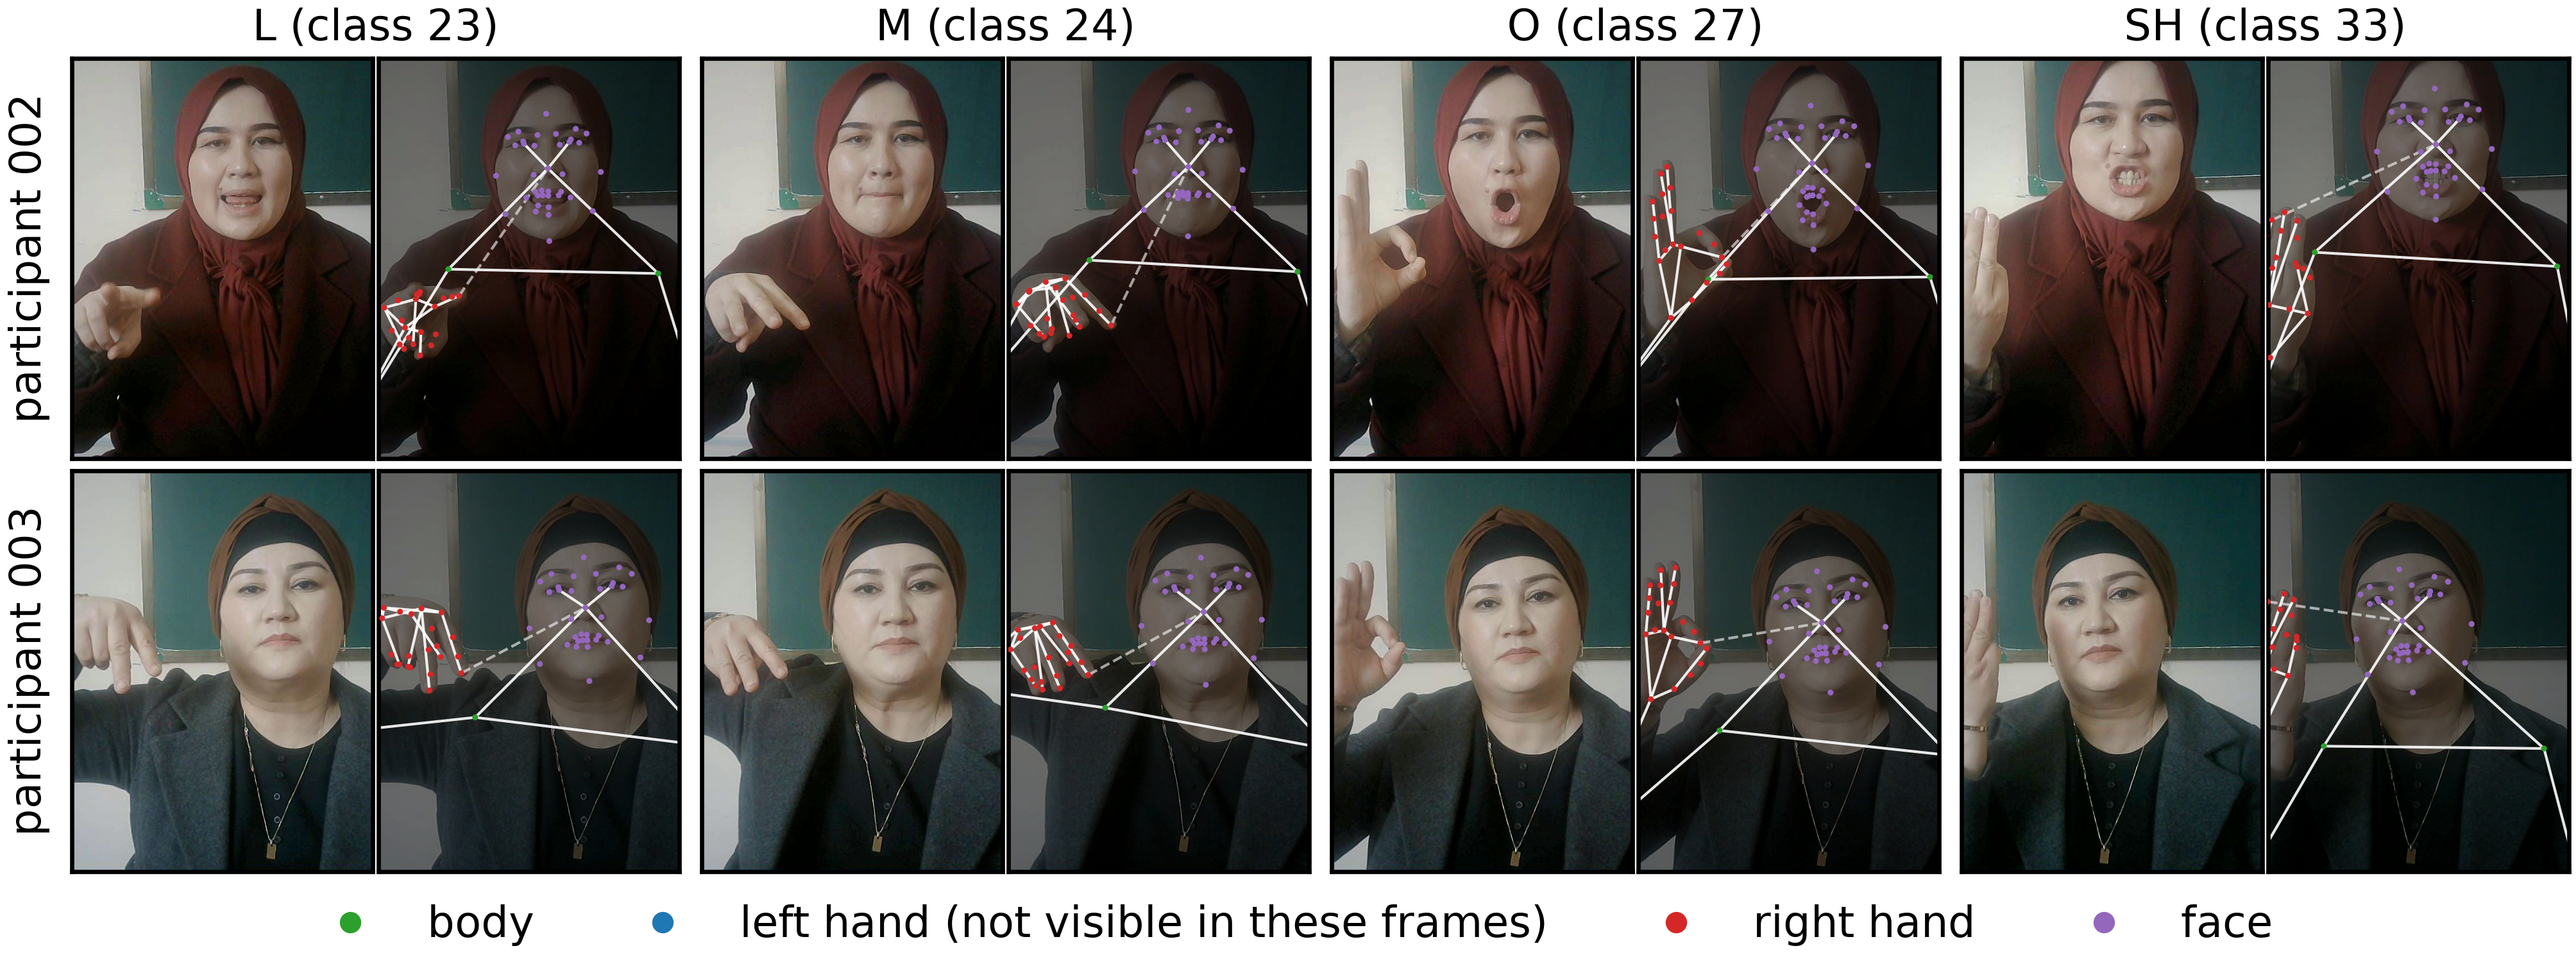
\includegraphics[width=\textwidth]{figures/fig1_signs.png}
\caption{Примеры знаков дактиля из пилота УзЖЯ: участники 002 и 003 (строки) и буквы L, M, O и SH (столбцы). Рядом с каждым кадром — тот же кадр с 85 точками и рёбрами графа из 27 узлов; дальние рёбра — пунктиром.}\label{fig:fig1_signs}
\end{figure*}

\begin{table*}[t]
\caption{Наборы данных. Видео «нет события» не учтены; 400 таких видео Slovo используются как дополнительный класс при обучении и валидации.}\label{tab:datasets}
\scriptsize\setlength{\tabcolsep}{3pt}
\centering
\begin{tabular}{lllrrrl}
\toprule
\textbf{Набор} & \textbf{Язык} & \textbf{Содержание} & \textbf{Видео} & \textbf{Классы} & \textbf{Исп.} & \textbf{Роль} \\
\midrule
Slovo & РЖЯ & изолированные слова & 20 000 & 1 000 & 194 & сравнение; предобучение \\
Bukva & РЖЯ & дактиль & 3 757 & 33 & 155 & сравнение; предобуч.; моделирование \\
Пилот УзЖЯ (наш) & УзЖЯ & дактиль, цифры & 322 & 40 & 3 & цель переноса \\
Корпус УзЖЯ (наш) & УзЖЯ & изолированные жесты (уроки + пилот) & 5 993 & 2 381 & 12 & LOSO; цель переноса \\
N01 (внешний) & УзЖЯ & видеословарь & 191 & 191 & 1 & только тест \\
imo-ishora.uz (внешний) & УзЖЯ & видеословарь & 1 556 & 1 556 & несколько & только тест \\
\bottomrule
\end{tabular}
\end{table*}

\hypertarget{ux43dux430ux431ux43eux440ux44b-ux434ux430ux43dux43dux44bux445-ux440ux443ux441ux441ux43aux43eux433ux43e-ux436ux435ux441ux442ux43eux432ux43eux433ux43e-ux44fux437ux44bux43aux430}{%
\subsection{Наборы данных русского жестового языка}\label{ux43dux430ux431ux43eux440ux44b-ux434ux430ux43dux43dux44bux445-ux440ux443ux441ux441ux43aux43eux433ux43e-ux436ux435ux441ux442ux43eux432ux43eux433ux43e-ux44fux437ux44bux43aux430}}

\textbf{Slovo} \citep{2023_kapitanov_slovo} содержит 20 000 видео 1 000 изолированных жестов РЖЯ, записанных 194 исполнителями, и 400 видео класса «нет события». Мы оставляем видео «нет события» дополнительным классом для обучения и валидации, поэтому у классификаторов Slovo 1 001 выход; наши тестовые наборы и официальное тестовое разбиение таких видео не содержат. \textbf{Bukva} \citep{2024_kvanchiani_bukva} содержит 3 757 видео 33 букв дактильной азбуки РЖЯ от 155 исполнителей; видео не обрезаны и размечены кадрами начала и конца жеста, используются только кадры между границами. Оба набора записаны многими исполнителями на разных устройствах в разнообразных условиях.

\hypertarget{ux43fux438ux43bux43eux442ux43dux44bux435-ux437ux430ux43fux438ux441ux438-ux443ux437ux436ux44f}{%
\subsection{Пилотные записи УзЖЯ}\label{ux43fux438ux43bux43eux442ux43dux44bux435-ux437ux430ux43fux438ux441ux438-ux443ux437ux436ux44f}}

Пилотный набор записан для этого исследования собственной программой при 1280 × 720 пикселей и 30 кадрах в секунду: 322 видео 40 дактильных знаков (29 букв узбекского алфавита на латинице, включая диграфы CH, SH и NG и буквы Gʻ и Oʻ, и числительные 0--10). Участник 001 --- второй автор, сделавший три пробные записи одной буквы при проверке программы; эти записи остаются в обучающих данных каждого фолда и никогда не тестируются. Участник 002 записал 143 видео 29 букв, участник 003 --- 176 видео 24 букв и 11 числительных, каждый за один сеанс в январе 2026 г. (0,30--3,67 с на видео, в среднем 1,24 с). У двух основных участников общие 24 буквы. Все участники дали письменное информированное согласие на запись, на использование данных в исследованиях и на публикацию изображений в научных статьях.

\hypertarget{ux43aux43eux440ux43fux443ux441-ux443ux437ux436ux44f-ux438ux437-ux43eux442ux43aux440ux44bux442ux44bux445-ux432ux438ux434ux435ux43eux443ux440ux43eux43aux43eux432}{%
\subsection{Корпус УзЖЯ из открытых видеоуроков}\label{ux43aux43eux440ux43fux443ux441-ux443ux437ux436ux44f-ux438ux437-ux43eux442ux43aux440ux44bux442ux44bux445-ux432ux438ux434ux435ux43eux443ux440ux43eux43aux43eux432}}

\textbf{Источники.} Мы отобрали открыто опубликованные видеоуроки УзЖЯ 11 каналов (162 урока, 15,23 ч), взяв только уроки, которые ведут взрослые; уроки с детьми исключены полностью. Записи дали десять каналов (159 уроков, 15,12 ч). Видео обрабатывались только на лабораторном компьютере, не распространяются и используются для внутренних исследований; каналы обозначены кодами C01--C11, ведущие --- кодами S01--S09. Два канала вёл один и тот же человек, и они объединены в одного исполнителя; три участника пилота --- S10--S12. Личность исполнителя устанавливалась по метаданным канала, а не распознаванием лиц, и ведущие разных каналов между собой не сравнивались.

\textbf{Сегментация.} Ключевые точки извлекались из всего урока (раздел 3.5). Для слов сегмент начинается, когда запястье поднимается выше уровня покоя (80-й процентиль минимальной высоты запястья минус 0,4 ширины плеч), и заканчивается, когда обе руки возвращаются; паузы короче 0,3 с объединяются, сегменты короче 0,4 с отбрасываются. Для дактиля и числительных сегмент --- удержание формы ведущей кисти (скорость изменения формы ниже двух размеров кисти в секунду не менее 0,32 с) внутри активного интервала. Автоматическая сегментация дала 11 153 сегмента.

\textbf{Разметка по трём признакам.} Сегмент получает метку, только если согласуются три независимых признака: текст на экране, распознанный Tesseract OCR \citep{2007_smith_tesseract} (модели узбекской латиницы или кириллицы) каждые 0,5 с с удалением логотипов, повторяющихся подписей и строк, похожих на субтитры; узбекская речь ведущего, транскрибированная моделью Whisper large-v3 \citep{2023_radford_whisper} и выровненная с сегментом в пределах ±2 с; и структура урока (слово, повторённое дважды подряд, или, в уроках дактиля, соответствие объявлений алфавиту). Названия видео не использовались. Сегмент принимается, если у него есть метка, правдоподобная физика рук (0,4--4 с, кисти видны не менее чем в 60 \% кадров, покой у границ) и не менее двух согласующихся признаков; остальные сегменты проходили автоматическую визуальную проверку отрисованных скелетов и вырезок текста мультимодальной языковой моделью (раздел 10) и отбрасывались, если были непригодны. После удаления 46 повторно загруженных дубликатов (корреляция траекторий запястий ≥ 0,9) и 314 сегментов, содержащих два или три жеста, осталась 5 671 запись уроков; вместе с 322 пилотными записями корпус содержит 5 993 записи 2 381 класса. Метки нормированы к узбекской латинице (апострофы, транслитерация с кириллицы, варианты написания сведены к самой частой форме); русские подписи переведены по словарю из 953 статей, не проверенному носителем языка, а синонимы и одинаковые буквы латиницы и кириллицы пока остаются отдельными классами (раздел 7).

\textbf{Точность меток.} Автоматические метки проверил второй автор слепым сравнением с эталонными видео онлайн-словаря УзЖЯ imo-ishora.uz (раздел 3.6). Из 300 случайных записей набора оценки (по 30 на исполнителя LOSO; затравка, правило сопоставления и правило подсчёта зафиксированы до проверки) эталон той же глоссы существовал для 113. Проверяющий видел сегмент корпуса рядом с эталоном, но не предсказания модели, и отвечал «тот же жест», «другой» или «не уверен». Метки совпали для 111 из 113 пар: 98,2 \% (95 \%-й ДИ {[}94,6; 100{]}, бутстреп по исполнителям); 57 из 57 пилотных пар и 54 из 56 пар уроков. Остальные 187 записей эталона не имели и оценивались по собственному знанию УзЖЯ проверяющим (182 «тот же», 3 «другой», 2 «не уверен»); этот подсчёт приводится только для сведения. Поскольку эталон имели лишь 56 записей уроков, измеренная точность относится к словам, которые есть в словаре, и получена одним проверяющим. Исключение пяти записей, оценённых как «другой», меняет точности LOSO не более чем на 0,1 пункта, поэтому все результаты ниже используют все записи.

\textbf{Состав и набор оценки.} Состав корпуса приведён в таблице 2. Почти весь словарь уроков --- слова; дактиль идёт в основном от участников пилота. Набор оценки содержит классы с не менее чем тремя записями от не менее чем двух исполнителей: 682 класса и 3 418 записей (3 146 слов, 272 буквы и числительных); 405 классов имеют трёх и более исполнителей, медианный класс --- четыре записи. Классы, записанные одним исполнителем (числительные пилота, буквы H, I, Q, V и Y и кириллический алфавит одного канала), участвуют в обучении, но никогда не тестируются.

\begin{table*}[t]
\caption{Состав корпуса УзЖЯ. «Набор оценки» — классы с ≥ 3 записями от ≥ 2 исполнителей (тест LOSO). Дактиль включает цифры.}\label{tab:corpus}
\footnotesize\setlength{\tabcolsep}{4pt}
\centering
\begin{tabular}{llrrcrrc}
\toprule
& & \multicolumn{3}{c}{\textbf{Все записи}} & \multicolumn{3}{c}{\textbf{Набор оценки}} \\ \cmidrule(lr){3-5}\cmidrule(lr){6-8}
\textbf{Исп.} & \textbf{Источник} & \textbf{Записей} & \textbf{Классов} & \textbf{Дактиль / слова} & \textbf{Записей} & \textbf{Классов} & \textbf{Дактиль / слова} \\
\midrule
S01 & C01 & 824 & 701 & 0 / 824 & 382 & 302 & 0 / 382 \\
S02 & C02 & 1 831 & 835 & 3 / 1828 & 1 095 & 446 & 3 / 1092 \\
S03 & C03 & 1 005 & 598 & 52 / 953 & 590 & 318 & 20 / 570 \\
S04 & C04 & 199 & 156 & 0 / 199 & 125 & 96 & 0 / 125 \\
S05 & C06 & 362 & 344 & 1 / 361 & 183 & 169 & 1 / 182 \\
S06 & C07 & 18 & 14 & 0 / 18 & 11 & 8 & 0 / 11 \\
S07 & C05, C08 & 1 146 & 979 & 13 / 1133 & 648 & 512 & 9 / 639 \\
S08 & C09 & 173 & 104 & 0 / 173 & 71 & 36 & 0 / 71 \\
S09 & C10 & 113 & 86 & 0 / 113 & 74 & 55 & 0 / 74 \\
S10 & пилот & 3 & 1 & 3 / 0 & 3 & 1 & 3 / 0 \\
S11 & пилот & 143 & 29 & 143 / 0 & 118 & 24 & 118 / 0 \\
S12 & пилот & 176 & 35 & 176 / 0 & 118 & 24 & 118 / 0 \\
Всего & 10 + пилот & 5 993 & 2 381 & 391 / 5602 & 3 418 & 682 & 272 / 3146 \\
\bottomrule
\end{tabular}
\end{table*}

\hypertarget{ux432ux43dux435ux448ux43dux438ux435-ux438ux441ux442ux43eux447ux43dux438ux43aux438}{%
\subsection{Внешние источники}\label{ux432ux43dux435ux448ux43dux438ux435-ux438ux441ux442ux43eux447ux43dux438ux43aux438}}

Для проверки использованы два источника, не участвовавшие в построении корпуса; итоговые модели были обучены до загрузки любого из них. \textbf{N01} --- открыто опубликованный видеословарь УзЖЯ с одним взрослым ведущим: 191 видео 191 жеста, размеченных по названиям видео (без проверки). \textbf{Онлайн-словарь imo-ishora.uz} содержит 1 556 эталонных видео изолированных жестов в исполнении нескольких взрослых ведущих, не встречающихся в корпусе; число ведущих не аннотировано. Оба источника используются только как тестовые наборы; их видео не входят в обучающие данные ни одной модели в этой статье.

\hypertarget{ux438ux437ux432ux43bux435ux447ux435ux43dux438ux435-ux43aux43bux44eux447ux435ux432ux44bux445-ux442ux43eux447ux435ux43a-ux438-ux43aux43eux43dux442ux440ux43eux43bux44c-ux43aux430ux447ux435ux441ux442ux432ux430}{%
\subsection{Извлечение ключевых точек и контроль качества}\label{ux438ux437ux432ux43bux435ux447ux435ux43dux438ux435-ux43aux43bux44eux447ux435ux432ux44bux445-ux442ux43eux447ux435ux43a-ux438-ux43aux43eux43dux442ux440ux43eux43bux44c-ux43aux430ux447ux435ux441ux442ux432ux430}}

Ключевые точки извлечены MediaPipe Holistic Landmarker 1.1.1 \citep{docs_mediapipe_holistic_landmarker} в видеорежиме со всеми порогами уверенности 0,5; для всех наборов использован один и тот же файл модели, идентифицируемый хешем SHA-256. Вслед за YouTube-ASL \citep{2023_uthus_youtube_asl} мы оставляем 85 из 553 точек: шесть точек позы (плечи, локти, бёдра), 2 × 21 точку кистей и 37 точек лица вокруг глаз, бровей, губ и контура лица, включая два центра радужек; используются только координаты изображения \(x\) и \(y\). Если кисть или лицо отсутствуют в части кадров, их координаты линейно интерполируются между ближайшими обнаруженными кадрами, а маска достоверности \(m\) для заполненных кадров равна 0; часть, ни разу не обнаруженная в клипе, обнуляется с \(m = 0\). Доля обнаружения кисти --- доля кадров с обнаруженной кистью среди кадров, где видно запястье, --- составила 79,1 \% на Slovo (80,5 \% в среднем по исполнителям, минимум 17,6 \%), 70,2 \% на Bukva и 94,3 \% на пилоте; поза тела найдена во всех кадрах Slovo и пилота. В корпусе хотя бы одна кисть обнаружена в среднем в 97,2 \% кадров (медиана 100 \%), обе кисти --- в 74,1 \%, лицо --- в 99,8 \%.

\hypertarget{ux44dux442ux438ux43aux430-ux438-ux437ux430ux449ux438ux442ux430-ux434ux430ux43dux43dux44bux445}{%
\subsection{Этика и защита данных}\label{ux44dux442ux438ux43aux430-ux438-ux437ux430ux449ux438ux442ux430-ux434ux430ux43dux43dux44bux445}}

Пилотные записи содержат лица и кисти участников и являются персональными данными; они не передаются. Видеоуроки открыто опубликованы их авторами; они использованы только для извлечения признаков и внутренней оценки, не распространяются, а извлечённые ключевые точки, позволяющие частично реконструировать исполнителя, не публикуются. Использование видеоуроков и видео словаря для исследований без их распространения подтверждено юридической службой Ферганского государственного университета (заключение № 32 от 5 ноября 2026 г.). ⟦Протокол исследования и использование пилотных записей одобрены ⟦этическим комитетом / учёным советом Ферганского государственного университета⟧, решение № ⟦\ldots⟧ от ⟦дата⟧.⟧

\hypertarget{ux43fux440ux43eux442ux43eux43aux43eux43bux44b-ux43eux446ux435ux43dux43aux438}{%
\section{Протоколы оценки}\label{ux43fux440ux43eux442ux43eux43aux43eux43bux44b-ux43eux446ux435ux43dux43aux438}}

\hypertarget{ux43fux440ux43eux442ux43eux43aux43eux43b-ux438ux437-ux43fux44fux442ux438-ux444ux43eux43bux434ux43eux432-ux441-ux43dux435ux43fux435ux440ux435ux441ux435ux43aux430ux44eux449ux438ux43cux438ux441ux44f-ux438ux441ux43fux43eux43bux43dux438ux442ux435ux43bux44fux43cux438-ux434ux43bux44f-ux440ux436ux44f-sd-5}{%
\subsection{Протокол из пяти фолдов с непересекающимися исполнителями для РЖЯ (SD-5)}\label{ux43fux440ux43eux442ux43eux43aux43eux43b-ux438ux437-ux43fux44fux442ux438-ux444ux43eux43bux434ux43eux432-ux441-ux43dux435ux43fux435ux440ux435ux441ux435ux43aux430ux44eux449ux438ux43cux438ux441ux44f-ux438ux441ux43fux43eux43bux43dux438ux442ux435ux43bux44fux43cux438-ux434ux43bux44f-ux440ux436ux44f-sd-5}}

Все сравнения на Slovo и Bukva используют пять фолдов с непересекающимися исполнителями (рис. 2а). На Slovo шесть исполнителей дают не менее 500 видео каждый и по правилу, зафиксированному до обучения, всегда относятся к обучающим данным; остальные 188 исполнителей делятся на пять групп, стратифицированных по числу записей, с фиксированной затравкой. В фолде \(k\) группа \(k\) --- тестовый набор, 10 \% исполнителей остальных групп образуют валидационный набор, остальные используются для обучения, так что каждый из 188 исполнителей (6 874 записи) тестируется ровно один раз. На Bukva так же делятся все 155 исполнителей. Перед каждым запуском код проверяет, что ни один исполнитель и ни одно видео не разделены между обучающими, валидационными и тестовыми данными и что все файлы точек получены одной и той же моделью разметки. Каждая конфигурация обучается с тремя случайными затравками на каждом фолде.

\begin{figure*}[t]
\centering
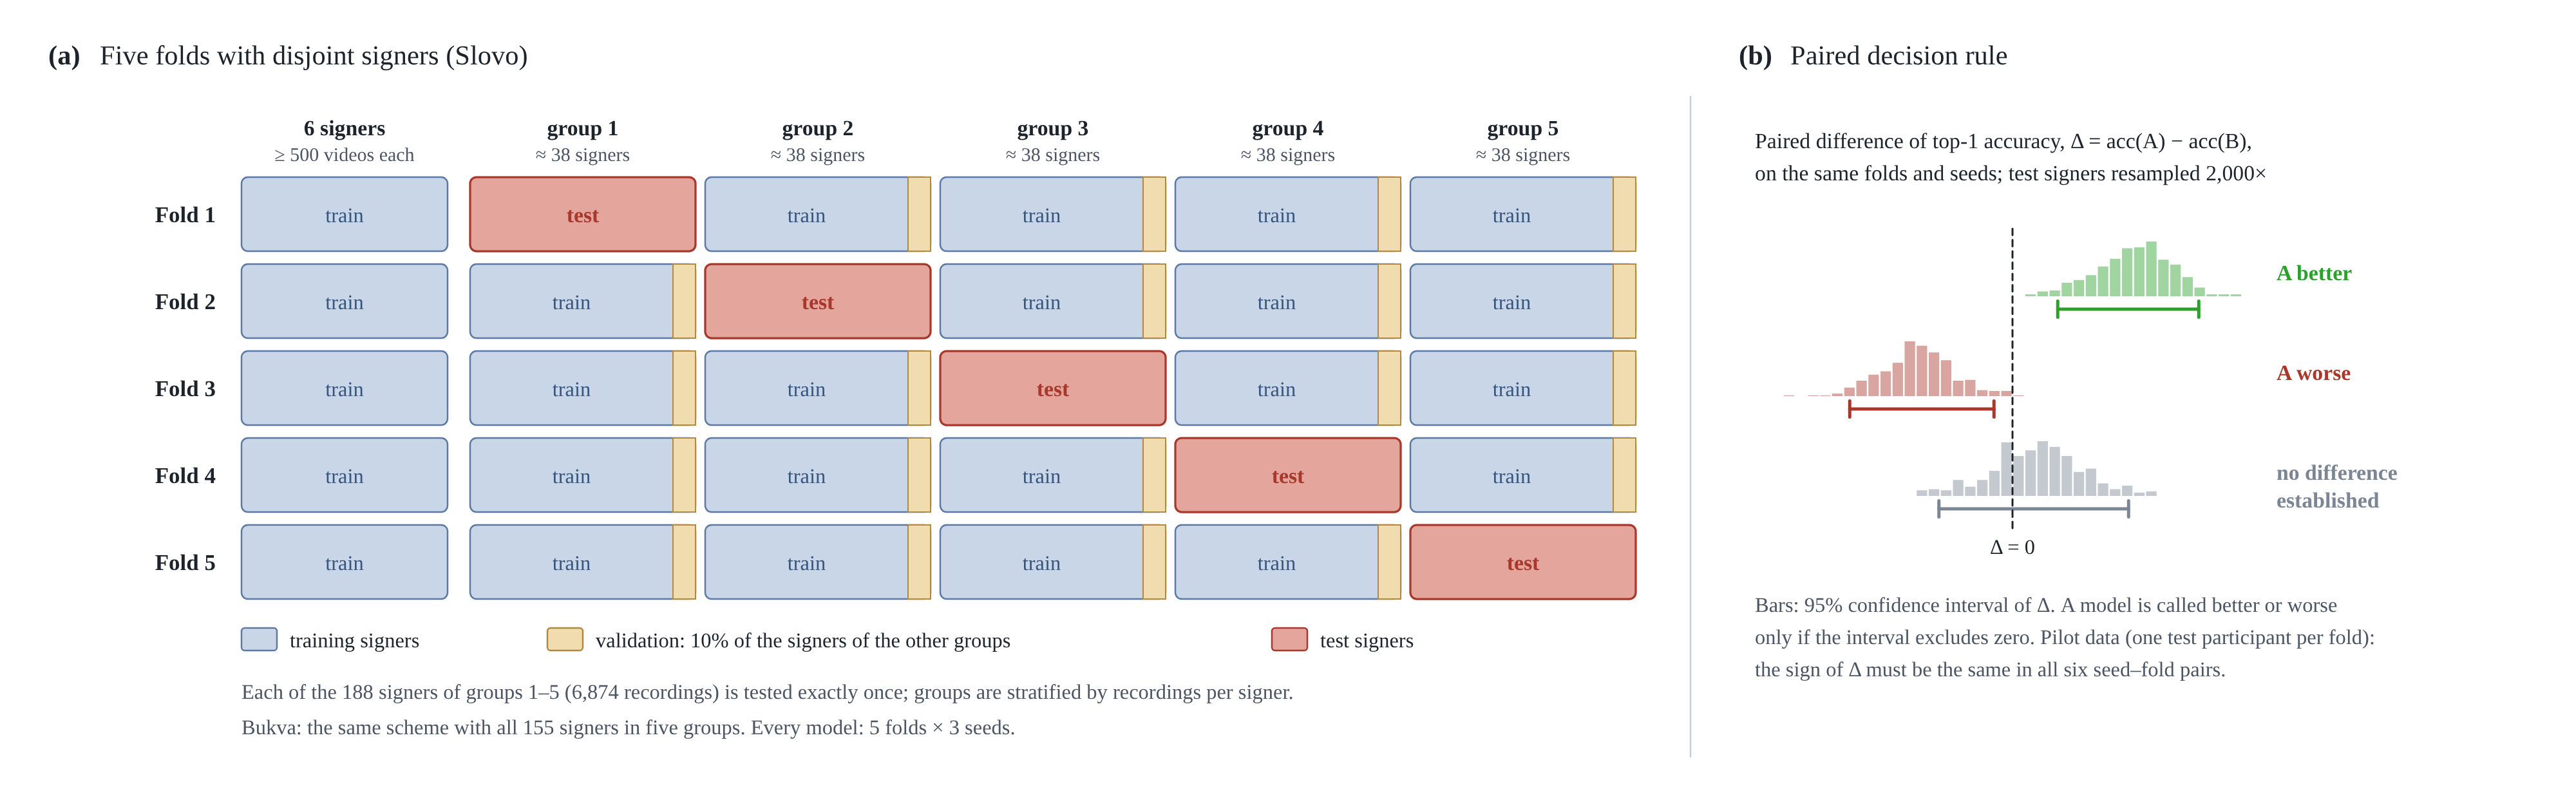
\includegraphics[width=\textwidth]{figures/fig2_protocol.png}
\caption{Протокол из пяти фолдов с непересекающимися исполнителями (SD-5). (а) Распределение по фолдам для Slovo: шесть исполнителей с ≥ 500 видео всегда в обучении; остальные 188 образуют пять групп, каждая один раз служит тестом, 10 \% исполнителей остальных групп — валидация. (б) Правило решения: модель лучше или хуже, только если 95 \%-й бутстреп-интервал парной разности по тестовым исполнителям не содержит нуля (распределения условные).}\label{fig:fig2_protocol}
\end{figure*}

\hypertarget{ux43fux440ux43eux442ux43eux43aux43eux43b-ux441-ux438ux441ux43aux43bux44eux447ux435ux43dux438ux435ux43c-ux43eux434ux43dux43eux433ux43e-ux438ux441ux43fux43eux43bux43dux438ux442ux435ux43bux44f-ux434ux43bux44f-ux43aux43eux440ux43fux443ux441ux430-ux443ux437ux436ux44f-loso}{%
\subsection{Протокол «с исключением одного исполнителя» для корпуса УзЖЯ (LOSO)}\label{ux43fux440ux43eux442ux43eux43aux43eux43b-ux441-ux438ux441ux43aux43bux44eux447ux435ux43dux438ux435ux43c-ux43eux434ux43dux43eux433ux43e-ux438ux441ux43fux43eux43bux43dux438ux442ux435ux43bux44f-ux434ux43bux44f-ux43aux43eux440ux43fux443ux441ux430-ux443ux437ux436ux44f-loso}}

Каждый из десяти исполнителей с не менее чем 20 записями набора оценки образует один тестовый фолд; два оставшихся исполнителя (14 записей) образуют дополнительный фолд, не включаемый в средние. Все остальные записи корпуса, включая классы с одной записью, используются для обучения, поэтому классификационная голова фолда имеет 682 класса, когда обучение ограничено набором оценки, и 2 033--2 378 классов, когда используются все записи. Валидационного набора нет: бюджеты обучения заданы заранее (раздел 5.4), и оцениваются веса последнего шага. Каждое условие запускается с тремя затравками, что даёт 33 запуска на модель. Поскольку у каждого ведущего уроков одна студия и одна камера, LOSO измеряет нового человека вместе с новыми условиями съёмки.

\hypertarget{ux43cux435ux442ux440ux438ux43aux438-ux438-ux43fux440ux430ux432ux438ux43bux430-ux440ux435ux448ux435ux43dux438ux44f}{%
\subsection{Метрики и правила решения}\label{ux43cux435ux442ux440ux438ux43aux438-ux438-ux43fux440ux430ux432ux438ux43bux430-ux440ux435ux448ux435ux43dux438ux44f}}

Основная метрика --- точность top-1. На SD-5 она объединяется по тестовым записям пяти фолдов и усредняется по затравкам; 95 \%-е доверительные интервалы получены бутстрепом по тестовым исполнителям (2 000 повторений) \citep{2016_efron_hastie_casi}. На LOSO это макросреднее по десяти тестовым исполнителям (точность каждого исполнителя усреднена по затравкам) с интервалами из 10 000 бутстреп-повторений по исполнителям; приводится и микросреднее по записям. Мы сообщаем точность top-5, макросреднее по исполнителям и точность худшего тестового исполнителя с не менее чем десятью записями на SD-5, а для всех наборов --- макроусреднённые по классам, присутствующим в тестовых данных, точность (precision), полноту и \(F_1\). Модель называется лучше или хуже другой, только если 95 \%-й доверительный интервал парной разности, вычисленной по тем же записям, затравкам и перевыбранным исполнителям, не содержит нуля; иначе мы сообщаем, что различие не установлено. На пилотных данных, где в каждом фолде один тестовый участник, различие сообщается, только если его знак одинаков во всех шести парах «затравка--фолд». Все правила решения, распределения по фолдам и бюджеты обучения были зафиксированы до соответствующих запусков.

\hypertarget{ux43cux43eux434ux435ux43bux438-ux438-ux43eux431ux443ux447ux435ux43dux438ux435}{%
\section{Модели и обучение}\label{ux43cux43eux434ux435ux43bux438-ux438-ux43eux431ux443ux447ux435ux43dux438ux435}}

\hypertarget{ux43cux43dux43eux433ux43eux44fux437ux44bux447ux43dux44bux439-ux43fux43eux437ux43eux432ux44bux439-ux43aux43eux434ux438ux440ux43eux432ux449ux438ux43a}{%
\subsection{Многоязычный позовый кодировщик}\label{ux43cux43dux43eux433ux43eux44fux437ux44bux447ux43dux44bux439-ux43fux43eux437ux43eux432ux44bux439-ux43aux43eux434ux438ux440ux43eux432ux449ux438ux43a}}

Многоязычный позовый кодировщик (МПК, рис. 3) принимает клип из \(T = 32\) кадров с 85 ключевыми точками в каждом и выдаёт \(D\)-мерное вложение клипа. Нормировка --- часть модели и экспортируется вместе с ней. После масштабирования координат \(y\) на соотношение сторон кадра каждая точка \(\mathbf{p}\) описывается в общей для всех точек системе координат тела, \[\mathbf{x}^{body} = \frac{1}{w}\,\mathbf{R}_{\theta}\,(\mathbf{p} - \mathbf{c}),\qquad(1)\] где \(\mathbf{c}\) --- середина отрезка между плечами, \(w\) --- ширина плеч, а \(\mathbf{R}_{\theta}\) поворачивает линию плеч в горизонтальное положение, причём \(\mathbf{c}\), \(w\) и \(\theta\) усреднены по клипу с маской позы в качестве весов, --- и в локальной системе координат, описывающей форму каждой кисти и лица независимо от их положения; для кисти \[\mathbf{x}^{loc} = \frac{\mathbf{p} - \mathbf{p}_{0}}{\lVert \mathbf{p}_{9} - \mathbf{p}_{0} \rVert},\qquad(2)\] где \(\mathbf{p}_0\) --- запястье, \(\mathbf{p}_9\) --- основание среднего пальца; для лица начало координат --- кончик носа, масштаб --- расстояние между центрами радужек, а поворот выравнивает радужки. Масштабы ограничены снизу величиной \(10^{-3}\), координаты обрезаются до \([-10, 10]\). Таким образом, каждая точка представлена шестью признаками \((x^{body}, y^{body}, x^{loc}, y^{loc}, m, c)\), где \(m\) --- маска достоверности, \(c\) --- уверенность детектора (видимость позы или флаг присутствия части).

\begin{figure*}[t]
\centering
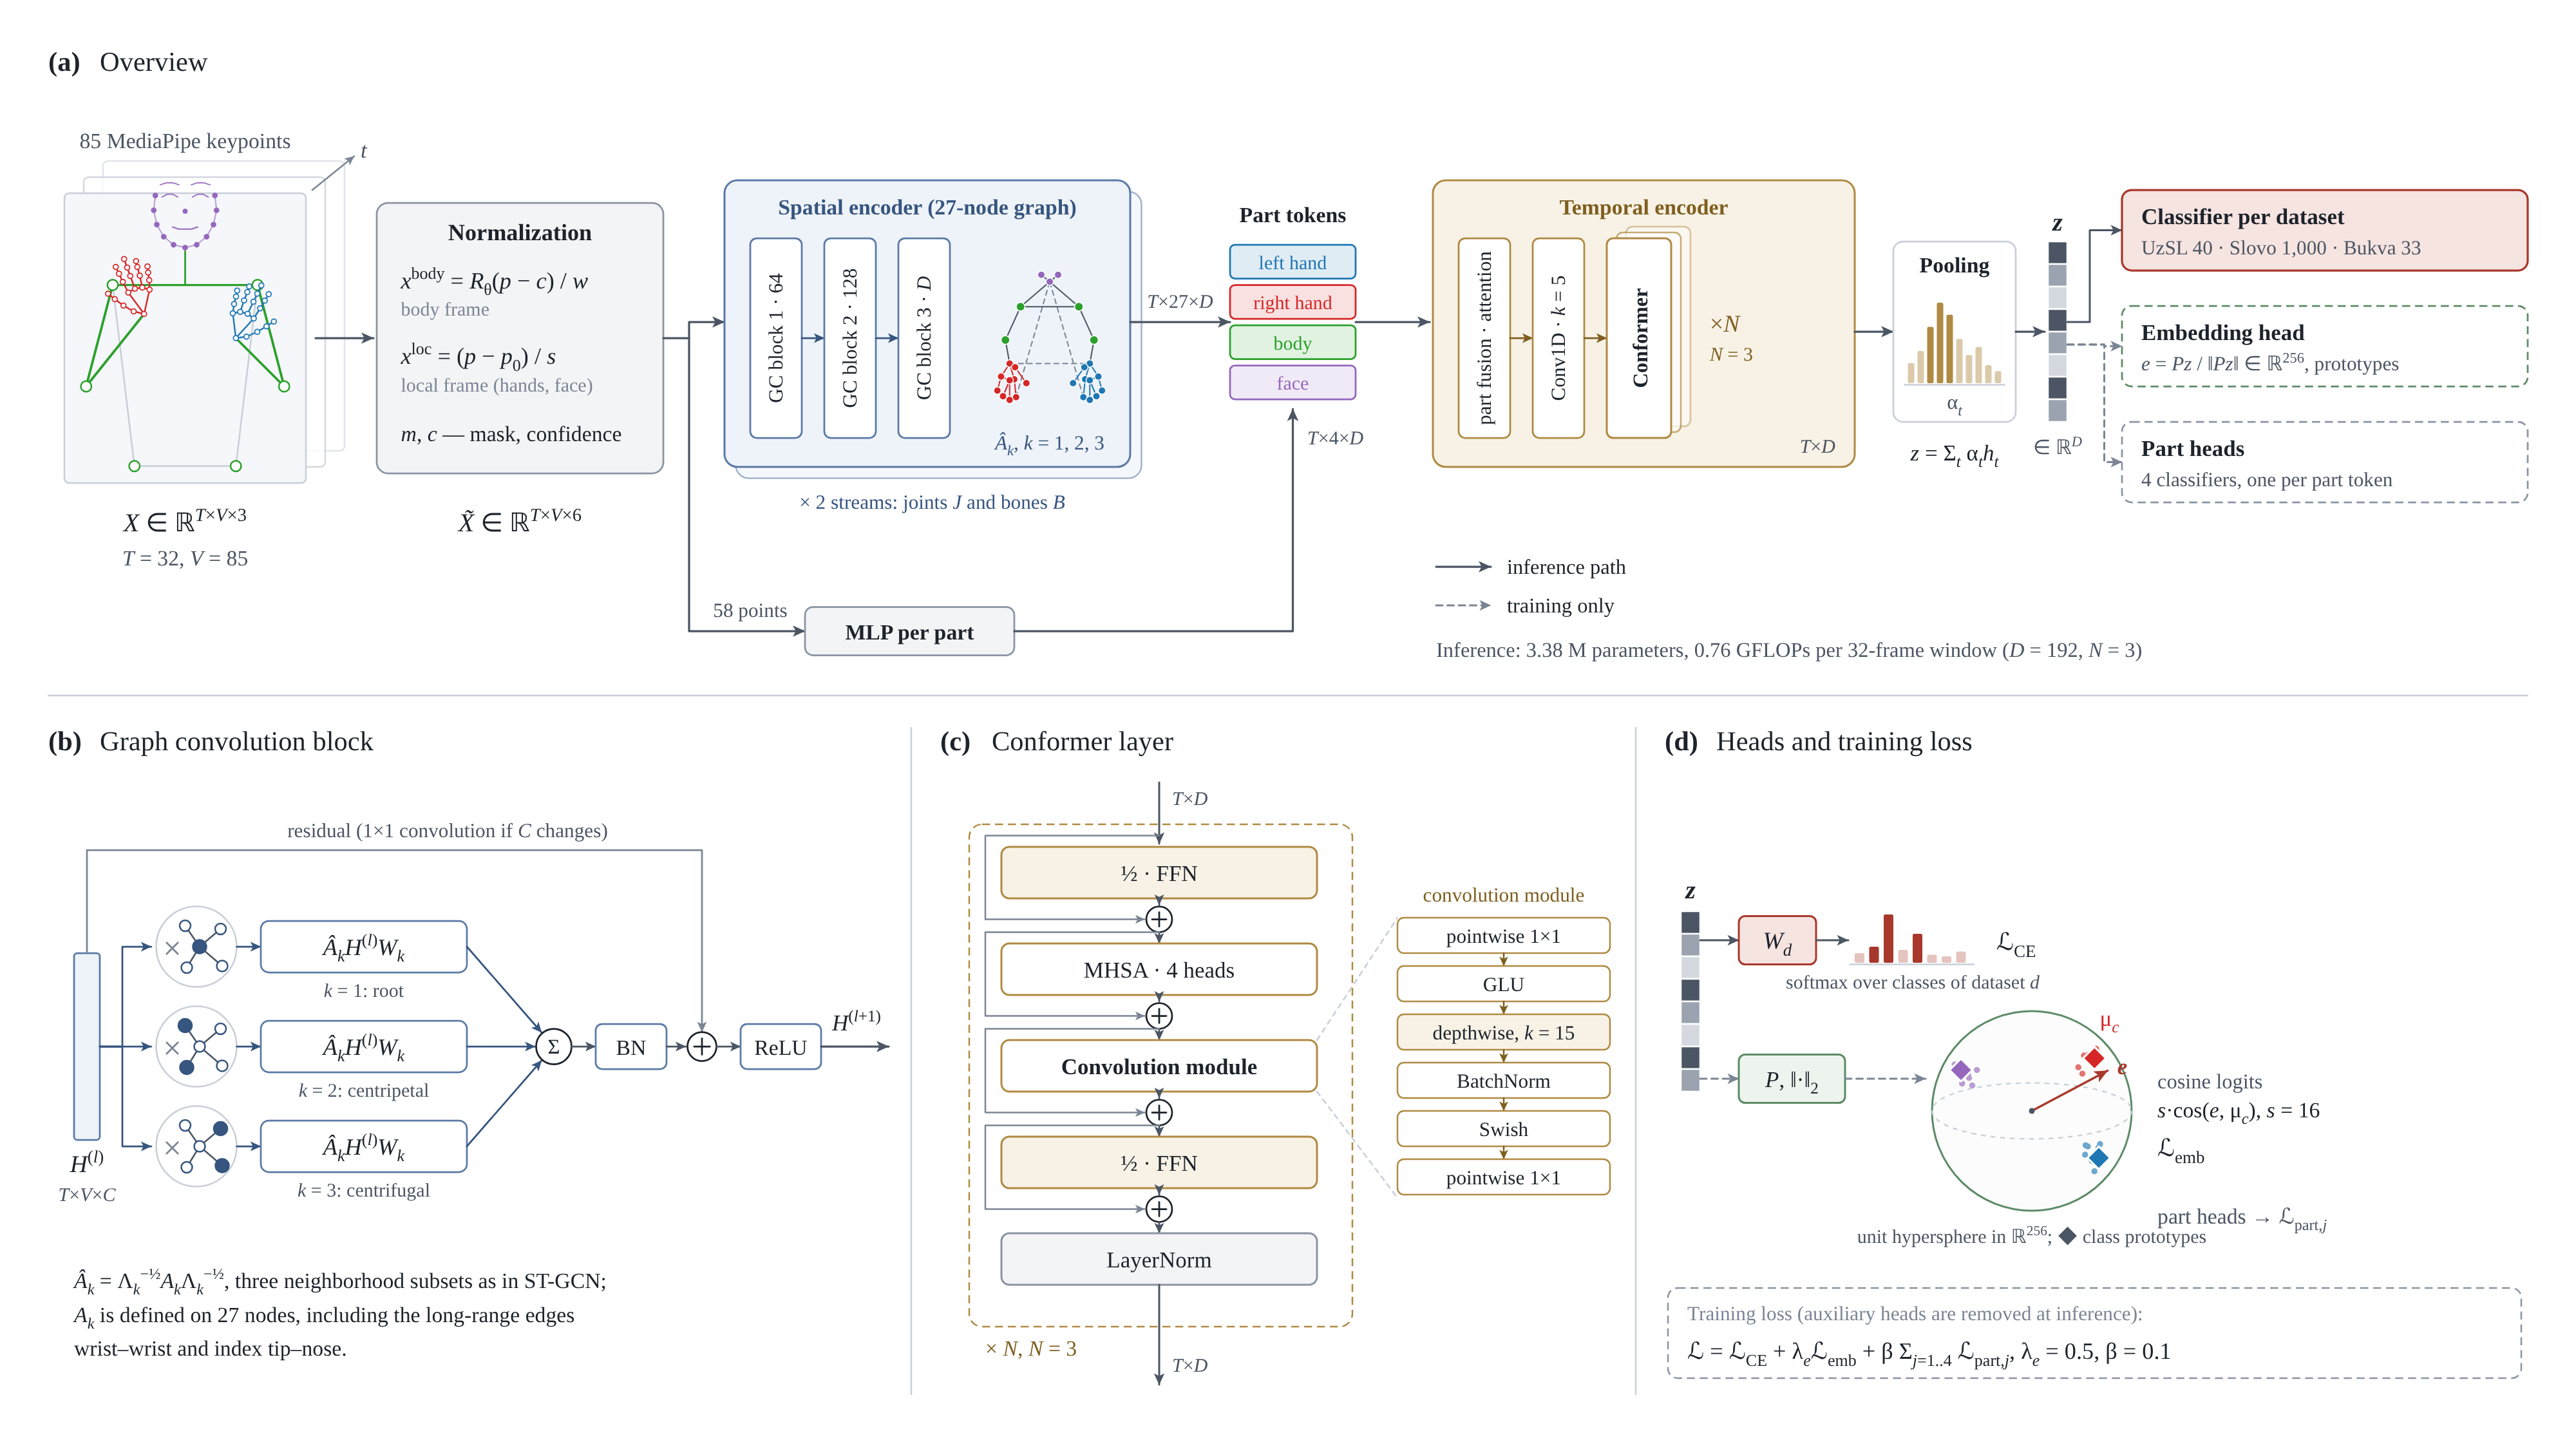
\includegraphics[width=\textwidth]{figures/fig3_architecture.png}
\caption{Архитектура многоязычного позового кодировщика (МПК). (а) Общая схема: нормировка, пространственный кодировщик на графе из 27 узлов с потоками суставов и костей, токены частей тела, временной кодировщик и пулинг вниманием; сплошные стрелки — путь распознавания, пунктир — головы только для обучения. (б) Блок графовой свёртки с тремя подмножествами окрестности. (в) Слой Conformer. (г) Классификационная голова для каждого набора и вспомогательные головы обучения.}\label{fig:fig3_architecture}
\end{figure*}

Подмножество из 27 точек образует граф: нос, два центра радужек, плечи и локти и десять точек каждой кисти (запястье, основание и кончик большого, указательного, среднего пальцев и мизинца и кончик безымянного пальца) с рёбрами тела вдоль рук, рёбрами кисти вдоль кинематической цепи и тремя дальними рёбрами, соединяющими два запястья и кончик каждого указательного пальца с носом. Вслед за ST-GCN \citep{2018_yan_stgcn} окрестность каждого узла делится на сам узел, соседей ближе к носу и соседей дальше от него, что даёт нормированные матрицы смежности \(\widehat{\mathbf{A}}_{k} = \mathbf{\Lambda}_{k}^{-1/2}\mathbf{A}_{k}\mathbf{\Lambda}_{k}^{-1/2}\), \(k = 1, 2, 3\), и блок графовой свёртки \[\mathbf{H}' = \mathrm{ReLU}\Big(\mathrm{BN}\Big(\sum_{k=1}^{3}\widehat{\mathbf{A}}_{k}\,\mathbf{H}\,\mathbf{W}_{k}\Big) + \mathrm{Res}(\mathbf{H})\Big),\qquad(3)\] где \(\mathrm{Res}\) --- тождественное отображение или проекция \(1 \times 1\). Три блока с 64, 128 и \(D\) каналами работают на каждом кадре; поток суставов и поток костей (разности между каждым узлом и его родителем в дереве с корнем в носе) суммируются поузлово.

Вложения 27 узлов и 58 точек вне графа группируются в четыре \emph{токена частей тела} на кадр --- левая кисть, правая кисть, тело и лицо; каждый токен --- сумма взвешенного по маске среднего вложений его узлов графа, двухслойного многослойного перцептрона (MLP) над шестью признаками его остальных точек и обучаемого вложения части; отсутствующая часть маскируется. Четыре токена объединяются вниманием с обучаемым запросом по присутствующим частям, добавляется обучаемое позиционное вложение, и последовательность проходит через поканальную временную свёртку (ядро 5) и \(N\) слоёв Conformer \citep{2020_gulati_conformer} (модули прямого распространения с половинным шагом и расширением 4, четырёхголовое самовнимание с маской кадров, свёрточный модуль с ядром 15, dropout 0,1). Пулинг вниманием по времени даёт вложение клипа \[\alpha_{t} = \operatorname{softmax}_{t}\big(\mathbf{w}^{\top}\tanh(\mathbf{W}\mathbf{h}_{t})\big),\qquad \mathbf{z} = \sum_{t=1}^{T}\alpha_{t}\,\mathbf{h}_{t}.\qquad(4)\] К \(\mathbf{z}\) присоединяется линейный классификатор для каждого набора данных; при совместном обучении на нескольких наборах каждый пример вносит перекрёстно-энтропийную потерю только через голову своего набора. Две вспомогательные головы используются только при обучении: нормированное 256-мерное вложение, обучаемое с косинусными логитами против обучаемых прототипов классов (масштаб 16), и по одному классификатору на каждый токен части, так что функция потерь при обучении \[\mathcal{L} = \mathcal{L}_{CE} + \lambda_{e}\,\mathcal{L}_{emb} + \beta\sum_{j=1}^{4}\mathcal{L}_{part,j},\qquad(5)\] при \(\lambda_e = 0{,}5\) и \(\beta = 0{,}1\).

Базовая конфигурация МПК-A0 использует \(D = 192\) и \(N = 3\): 4,41 млн параметров при обучении и 3,38 млн при выводе, 0,76 GFLOPs на окно из 32 кадров (подсчёт \texttt{torch.utils.flop\_counter}, умножение-сложение как две операции). Основная конфигурация МПК-A1 добавляет экспоненциальное скользящее среднее (EMA) весов для валидации и тестирования \citep{1992_polyak_averaging} с коэффициентом 0,999 при бюджетах от 3 000 шагов и 0,99 иначе; МПК-A2 заменяет блоки графовой свёртки MLP по частям (3,14 млн параметров, 0,196 GFLOPs). Увеличенный вариант с \(D = 256\) и \(N = 6\) (10,27 млн параметров, 1,33 GFLOPs) используется в исследовании ёмкости.

\hypertarget{ux431ux430ux437ux43eux432ux44bux435-ux43cux43eux434ux435ux43bux438}{%
\subsection{Базовые модели}\label{ux431ux430ux437ux43eux432ux44bux435-ux43cux43eux434ux435ux43bux438}}

Все базовые модели получают те же файлы точек и фолды. \textbf{ST-GCN} \citep{2018_yan_stgcn} и \textbf{SL-GCN} \citep{2021_jiang_sam_slr} запускаются из кода, опубликованного их авторами (репозиторий yysijie/st-gcn, коммит 221c0e15; поток суставов кода SAM-SLR, коммит de6c53a6), на наших 27 точках --- как внутри нашего цикла обучения с общим рецептом (ниже) и окном в 32 кадра (3,34 и 5,07 млн параметров; 1,98 и 2,19 GFLOPs), так и с конфигурациями обучения их авторов (для SL-GCN: SGD, 250 эпох, случайные окна в 100 кадров при обучении и 150 кадров при тестировании, DropGraph; для ST-GCN: конфигурация его репозитория, тестирующая на буфере из 300 кадров). Наши более ранние реализации обеих сетей на графе из 27 узлов и входных признаках МПК приводятся для сравнения, но не используются как базовые модели по причине, изложенной в разделе 6.1. \textbf{Трансформер по ключевым точкам} --- трансформер-кодировщик с предварительной нормализацией \citep{2017_vaswani_attention} и токеном классификации над 67 точками на кадр (25 точек верхней части тела и обе кисти), \(D = 256\), четыре слоя и окно в 64 кадра (3,53 млн параметров, 0,43 GFLOPs), обученный с общим рецептом и с рецептом, разработанным для него ранее (выбранным на валидационных данных); приводится лучший рецепт. Три простые базовые модели --- двухслойный трансформер, двунаправленная LSTM с пулингом вниманием и MLP --- используют общий рецепт без усреднения весов. \textbf{MViTv2-S} \citep{2022_li_mvitv2}, видеомодель, опубликованная вместе со Slovo, оценивается только на официальном разбиении Slovo как ориентир.

\hypertarget{ux43eux431ux449ux438ux439-ux440ux435ux446ux435ux43fux442-ux43eux431ux443ux447ux435ux43dux438ux44f}{%
\subsection{Общий рецепт обучения}\label{ux43eux431ux449ux438ux439-ux440ux435ux446ux435ux43fux442-ux43eux431ux443ux447ux435ux43dux438ux44f}}

Все модели по ключевым точкам обучаются с AdamW (скорость обучения \(10^{-3}\), затухание весов 0,05), линейным разогревом на 5 \% шагов и косинусным убыванием до нуля, сглаживанием меток 0,1, размером пакета 128 и смешанной точностью bfloat16; потеря прототипных вложений входит в общий рецепт для всех моделей, тогда как головы частей есть только у МПК. Бюджеты задаются в шагах оптимизатора и одинаковы для всех моделей, сравниваемых на наборе: \(\lceil 100\,N_{train}/128 \rceil\), где \(N_{train}\) --- наибольший обучающий набор среди фолдов (14 488 шагов на Slovo, 2 154 на Bukva, около 100 эпох). При обучении окно из 32 кадров выбирается со случайным темпом от ×0,5 до ×2; кадры выбрасываются с вероятностью 0,1 и дублируются с вероятностью 0,3, границы жеста сдвигаются до пяти кадров, кисть удаляется в 20--25 \% кадров, а точки поворачиваются (±15°), масштабируются (0,9--1,1), сдвигаются (±0,05 ширины кадра) и, для кистей, зашумляются гауссовым шумом (\(\sigma\) = 0,002). При тестировании 32 кадра выбираются равномерно по клипу. Контрольная точка с лучшей валидационной точностью top-1 тестируется один раз; затравки 0, 1 и 2 управляют инициализацией, порядком пакетов и аугментацией. Все модели обучены на одной NVIDIA GeForce RTX 5080 (16 ГБ) с PyTorch 2.14.1; один запуск МПК-A1 на Slovo занимает около 4 мин. Обучение на GPU не детерминировано побитово, и повторный запуск конфигурации меняет результат примерно так же, как смена затравки.

\hypertarget{ux43fux435ux440ux435ux43dux43eux441-ux43dux430-ux443ux437ux436ux44f-ux438-ux431ux44eux434ux436ux435ux442ux44b-ux437ux430ux434ux430ux43dux43dux44bux435-ux437ux430ux440ux430ux43dux435ux435}{%
\subsection{Перенос на УзЖЯ и бюджеты, заданные заранее}\label{ux43fux435ux440ux435ux43dux43eux441-ux43dux430-ux443ux437ux436ux44f-ux438-ux431ux44eux434ux436ux435ux442ux44b-ux437ux430ux434ux430ux43dux43dux44bux435-ux437ux430ux440ux430ux43dux435ux435}}

Сравниваются три источника предобучения --- Slovo, Bukva и оба вместе с раздельными головами; кодировщик предобучается на всех записях источника с 5 \% исполнителей источника, отложенными для выбора контрольной точки. На целевых данных сравниваются три схемы: обучение с нуля, полное дообучение (кодировщик заморожен первые 20 \% шагов, затем размораживается послойно каждые 7 \% шагов, скорость обучения основы --- 0,1 скорости головы) и линейный зонд с замороженным кодировщиком. При двух-трёх участниках валидационный набор из записей обучающих участников измеряет не то (раздел 6.6), поэтому бюджеты обучения были заданы до любого запуска на пилоте или корпусе по моделированию на Bukva под SD-5 с четырьмя записями на класс: бюджет --- медиана по 15 запускам шага с лучшей валидационной точностью, 1 466,2 эпохи для обучения с нуля и 209,5 эпохи для дообучения и линейного зонда. На целевых данных число шагов равно \(\lceil \text{эпохи} \times N_{train}/128 \rceil\), оценивается модель последнего шага, целевые данные не используются для выбора модели, а бюджеты были зафиксированы в системе контроля версий до первого запуска. Для коротких запусков коэффициент EMA разогревается как \(\min(0{,}99, (1+t)/(10+t))\) на шаге \(t\). На пилоте каждое условие запускается с тремя затравками на обоих фолдах (тестовый участник 002 или 003), предобучение повторяется для каждой затравки; на корпусе те же бюджеты дают 5 389 шагов для предобученных моделей с обучающим набором из 682 классов, 9 482 --- со всеми записями, и 37 720 и 66 368 шагов для обучения с нуля. Оригинальный SL-GCN переносился с точно теми же фолдами, рецептом и бюджетами после собственного предобучения на Slovo и Bukva.

\hypertarget{ux440ux435ux437ux443ux43bux44cux442ux430ux442ux44b}{%
\section{Результаты}\label{ux440ux435ux437ux443ux43bux44cux442ux430ux442ux44b}}

Все точности --- top-1 в процентах, если не указано иное; в квадратных скобках --- 95 \%-е доверительные интервалы по исполнителям; \(\Delta\) обозначает парную разность. Каждое число этого раздела вычислено из предсказаний запусков по отдельным записям одним скриптом, опубликованным вместе с кодом.

\hypertarget{ux43cux43eux434ux435ux43bux438-ux43fux43e-ux43aux43bux44eux447ux435ux432ux44bux43c-ux442ux43eux447ux43aux430ux43c-ux43dux430-ux440ux443ux441ux441ux43aux43eux43c-ux436ux435ux441ux442ux43eux432ux43eux43c-ux44fux437ux44bux43aux435}{%
\subsection{Модели по ключевым точкам на русском жестовом языке}\label{ux43cux43eux434ux435ux43bux438-ux43fux43e-ux43aux43bux44eux447ux435ux432ux44bux43c-ux442ux43eux447ux43aux430ux43c-ux43dux430-ux440ux443ux441ux441ux43aux43eux43c-ux436ux435ux441ux442ux43eux432ux43eux43c-ux44fux437ux44bux43aux435}}

Таблица 3 сравнивает модели по SD-5, рис. 4 соотносит точность с объёмом вычислений. МПК-A1 достигает 70,8 \% на Slovo и 93,2 \% на Bukva. Он точнее трансформера по ключевым точкам на 4,4 пункта на Slovo и на 8,1 пункта на Bukva, а простые базовые модели отстают на 8,6--42,2 пункта. Оригинальные ST-GCN и SL-GCN, обученные с тем же рецептом и окном, точнее на Slovo: 73,1 \% и 74,4 \%, \(\Delta\) = +2,3 {[}+1,3; +3,4{]} и +3,7 {[}+2,5; +4,8{]} относительно МПК-A1, при в 2,6 и 2,9 раза большем числе операций на окно. На Bukva при общем рецепте и окне оригинальные сети достигают 87,4 \% и 89,6 \% --- на 5,8 {[}−6,6; −4,9{]} и 3,5 пункта {[}−4,5; −2,7{]} ниже МПК-A1; SL-GCN с рецептом авторов так же точен, как МПК-A1 (93,1 \% против 93,2 \%, \(\Delta\) = −0,1 {[}−0,9; +0,7{]}), при в 12,8 раза большем числе операций на клип, а ST-GCN с рецептом авторов намного слабее (68,8 \%). Макроусреднённые по классам точность (precision), полнота и \(F_1\) лежат на 2--3 пункта ниже точности top-1 на Slovo и в пределах одного пункта от неё на Bukva, а порядок моделей по \(F_1\) совпадает с порядком по top-1. Макросреднее по исполнителям на Slovo до 4 пунктов ниже объединённой точности, а худший тестовый исполнитель с не менее чем десятью записями достигает для МПК-A1 лишь 27 \% (71 \% на Bukva), так что все модели сильно отстают на части исполнителей.

\begin{table*}[t]
\caption{Модели по ключевым точкам по протоколу SD-5: точность top-1 и top-5, macro-усреднённые по классам точность (precision), полнота и $F_1$, парная разность top-1 с МПК-A1 (95 \% ДИ по тестовым исполнителям). Строки без пометки — три затравки × пять фолдов; † — оригинальный код или рецепт, одна затравка; * — общий рецепт без усреднения весов. Параметры и GFLOPs даны один раз, для моделей Slovo на окне проверки (32 кадра; 64 — трансформер по точкам; 150 — рецепт SL-GCN; 300 — ST-GCN с рецептом авторов); задержки на ЦП — в тексте.}\label{tab:rsl_main}
\scriptsize\setlength{\tabcolsep}{2pt}
\centering
\begin{tabular}{lrrlrrrrl}
\toprule
\textbf{Модель} & \textbf{Парам., млн} & \textbf{GFLOPs} & \textbf{Top-1 [95 \% ДИ]} & \textbf{Top-5} & \textbf{Точность} & \textbf{Полнота} & \textbf{$F_1$} & \textbf{$\Delta$ top-1 с МПК-A1 [95 \% ДИ]} \\
\midrule
\multicolumn{9}{l}{\textit{Slovo (1 000 классов, 188 тестовых исполнителей)}} \\
МПК-A1 & 3,38 & 0,76 & 70,8 [68,8; 72,7] & 92,1 & 70,4 & 69,8 & 68,7 & --- \\
ST-GCN, оригинал † & 3,34 & 1,98 & 73,1 [71,4; 74,7] & 93,2 & 73,1 & 72,2 & 71,3 & +2,3 [+1,3; +3,4] \\
SL-GCN, оригинал † & 5,07 & 2,19 & 74,4 [72,4; 76,3] & 94,0 & 74,4 & 73,6 & 72,6 & +3,7 [+2,5; +4,8] \\
ST-GCN, оригинал, рецепт авторов † & 3,34 & 18,54 & 61,6 [59,1; 64,1] & 87,4 & 61,0 & 60,5 & 59,1 & −9,2 [−10,6; −7,7] \\
SL-GCN, оригинал, рецепт авторов † & 5,07 & 9,70 & 74,6 [72,7; 76,4] & 93,3 & 74,4 & 73,7 & 72,9 & +3,8 [+2,8; +5,1] \\
МПК-A1, рецепт SL-GCN † & 3,40 & 3,59 & 71,2 [69,0; 73,2] & 90,9 & 71,1 & 70,5 & 69,3 & +0,4 [−0,5; +1,3] \\
ST-GCN, наша реализация & 3,41 & 1,98 & 69,0 [67,0; 70,8] & 91,3 & 68,9 & 67,8 & 66,8 & −1,8 [−2,7; −1,1] \\
SL-GCN, наша реализация & 3,93 & 2,03 & 68,1 [66,2; 69,8] & 91,9 & 67,3 & 67,2 & 65,7 & −2,7 [−3,4; −2,0] \\
Трансформер по точкам & 3,53 & 0,43 & 66,3 [64,1; 68,3] & 89,0 & 65,9 & 65,4 & 64,0 & −4,4 [−5,7; −3,2] \\
Двухслойный трансформер * & 1,98 & 0,11 & 56,4 [54,1; 58,6] & 81,0 & 56,0 & 55,4 & 53,7 & −14,4 [−15,7; −13,2] \\
BiLSTM с вниманием * & 11,00 & 0,62 & 52,3 [49,9; 54,7] & 77,4 & 51,1 & 51,2 & 49,3 & −18,4 [−19,8; −17,2] \\
MLP * & 1,55 & 0,004 & 28,6 [26,7; 30,4] & 55,5 & 28,0 & 27,5 & 25,3 & −42,2 [−43,8; −40,6] \\
\multicolumn{9}{l}{\textit{Bukva (33 класса, 155 тестовых исполнителей)}} \\
МПК-A1 &  &  & 93,2 [92,3; 94,0] & 99,4 & 93,2 & 93,1 & 93,1 & --- \\
ST-GCN, оригинал † &  &  & 87,4 [86,3; 88,5] & 99,3 & 87,5 & 87,4 & 87,4 & −5,8 [−6,6; −4,9] \\
SL-GCN, оригинал † &  &  & 89,6 [88,4; 90,7] & 99,4 & 89,8 & 89,6 & 89,7 & −3,5 [−4,5; −2,7] \\
ST-GCN, оригинал, рецепт авторов † &  &  & 68,8 [67,1; 70,5] & 98,2 & 68,6 & 68,3 & 67,5 & −24,4 [−26,0; −22,7] \\
SL-GCN, оригинал, рецепт авторов † &  &  & 93,1 [91,9; 94,1] & 99,4 & 93,1 & 93,0 & 93,0 & −0,1 [−0,9; +0,7] \\
ST-GCN, наша реализация &  &  & 78,7 [77,4; 80,0] & 99,2 & 78,9 & 78,6 & 78,5 & −14,5 [−15,6; −13,4] \\
SL-GCN, наша реализация &  &  & 84,9 [83,9; 86,0] & 99,3 & 85,2 & 84,7 & 84,4 & −8,3 [−9,1; −7,3] \\
Трансформер по точкам &  &  & 85,1 [82,7; 87,2] & 96,4 & 85,4 & 85,0 & 85,1 & −8,1 [−10,2; −6,2] \\
Двухслойный трансформер * &  &  & 75,4 [72,8; 77,9] & 92,5 & 75,7 & 75,4 & 75,2 & −17,8 [−20,3; −15,5] \\
BiLSTM с вниманием * &  &  & 84,6 [83,2; 85,8] & 98,3 & 84,7 & 84,5 & 84,6 & −8,6 [−9,7; −7,7] \\
MLP * &  &  & 70,9 [68,9; 72,7] & 97,6 & 70,9 & 70,4 & 70,1 & −22,3 [−23,9; −20,7] \\
\bottomrule
\end{tabular}
\end{table*}

\begin{figure*}[t]
\centering
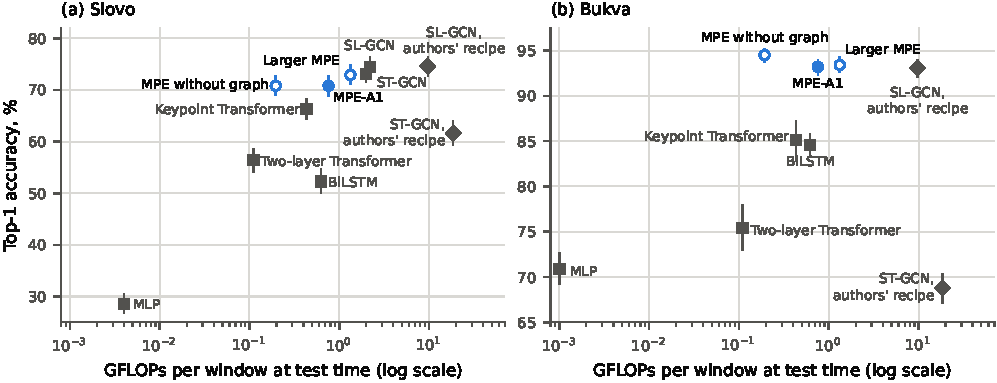
\includegraphics[width=\textwidth]{figures/fig5_cost.pdf}
\caption{Точность top-1 по SD-5 и объём вычислений на окно при проверке (логарифмическая шкала): (а) Slovo, (б) Bukva. Закрашенный круг — МПК-A1; незакрашенные — МПК-A2 и большая МПК; квадраты — базовые с общим рецептом (ST-GCN и SL-GCN — оригинальный код, только Slovo); ромбы — оригинальный код с рецептами авторов. Отрезки — 95 \% ДИ по исполнителям.}\label{fig:fig5_cost}
\end{figure*}

\textbf{Переписанные базовые модели занижают оригинальный код.} Сначала мы сами реализовали ST-GCN и SL-GCN на графе из 27 узлов и входных признаках МПК. С общим рецептом они достигли 69,0 \% и 68,1 \% на Slovo --- на 4,1 {[}+3,1; +5,2{]} и 6,4 {[}+5,4; +7,3{]} пункта ниже оригинального кода, обученного с тем же рецептом, а на Bukva наши ST-GCN и SL-GCN достигли 78,7 \% и 84,9 \% --- на 8,7 {[}+7,5; +9,9{]} и 4,7 пункта {[}+3,7; +5,7{]} ниже оригинального кода при том же рецепте (и на 8,1 пункта ниже SL-GCN с рецептом авторов). Наши реализации упрощали исходные блоки (для SL-GCN --- развязанную графовую свёртку, пространственно-временно-канальное внимание и DropGraph; для ST-GCN --- нормировку окрестности, входные каналы и dropout) и их инициализацию. Сравни мы МПК только с этими реализациями, он выглядел бы на 1,8--2,7 пункта \emph{лучше} графовых сетей вместо 2,3--3,7 пункта хуже. Рецепт не объясняет силу SL-GCN на Slovo: с рецептом авторов он достигает 74,6 \%, столько же, сколько с общим рецептом (\(\Delta\) = +0,2 {[}−1,0; +1,3{]}), а МПК-A1, обученный с рецептом SL-GCN и окнами в 150 кадров, ничего не выигрывает (71,2 \%, +0,4 {[}−0,6; +1,3{]}) и остаётся на 3,5 пункта ниже SL-GCN при этом рецепте, ниже на всех пяти фолдах. На Bukva рецепт значит больше: SL-GCN выигрывает от рецепта авторов 3,4 пункта {[}+2,4; +4,4{]}, а ST-GCN теряет 18,6 пункта с конфигурацией своего репозитория. Трансформер по ключевым точкам, напротив, выиграл от собственного рецепта 3,9 пункта {[}+2,7; +5,2{]}, поэтому он приводится с ним. Оригинальный ST-GCN с конфигурацией своего репозитория намного слабее на обоих наборах (61,6 \% на Slovo, 68,8 \% на Bukva); возможные причины (короткое расписание, вход без нормировки кистей) мы не разделяли.

\textbf{Стоимость.} По числу операций с плавающей точкой МПК-A1 дешевле обеих графовых сетей, но на настольном ЦП (Intel Core i9-14900KF, float32, пакет 1, медиана 100 запусков после 10 прогревочных, eager PyTorch) он не быстрее ST-GCN: 8,4--9,3 мс против 5,7 мс, тогда как оригинальному SL-GCN нужны 23,0 мс. Мы объясняем это множеством мелких операций МПК (два потока, токены частей, Conformer), которые eager-режим выполняет менее эффективно, чем несколько крупных свёрток. При экспорте в ONNX и запуске в ONNX Runtime 1.31 на том же ЦП (обученные веса, один поток, медиана 100 запусков; измерено при машине, частично занятой обучением, то есть верхняя оценка) порядок меняется: МПК-A1 занимает 10,8 мс, оригинальный ST-GCN --- 15,0 мс, оригинальный SL-GCN --- 25,6 мс, МПК-A2 --- 1,8 мс (7,2, 7,6, 19,3 и 1,0 мс при четырёх потоках). Задержки одной и той же модели различались между сеансами на 1--2 мс и сравниваются только по порядку величины; экспортированные модели описаны в разделе 6.7.

\hypertarget{ux447ux442ux43e-ux43eux43fux440ux435ux434ux435ux43bux44fux435ux442-ux442ux43eux447ux43dux43eux441ux442ux44c}{%
\subsection{Что определяет точность}\label{ux447ux442ux43e-ux43eux43fux440ux435ux434ux435ux43bux44fux435ux442-ux442ux43eux447ux43dux43eux441ux442ux44c}}

Рис. 5 показывает абляции МПК-A1 (три затравки × пять фолдов, парные разности). Замена четырёх токенов частей одним токеном на кадр снижает точность на 2,7 пункта {[}−3,3; −2,0{]} на Slovo и на 5,7 пункта {[}−6,9; −4,7{]} на Bukva --- единственное изменение, вредящее на обоих наборах. Замена графовых свёрток MLP по частям (МПК-A2) не меняет точность на Slovo (+0,0 {[}−0,7; +0,7{]}) и улучшает Bukva на 1,3 пункта {[}+0,8; +1,8{]}, сокращая вычисления в 3,9 раза. Удаление дальних рёбер стоит 0,9 пункта на Slovo, но даёт 0,6 на Bukva; граф без них хуже, чем отсутствие графа. Усреднение весов добавляет 1,5 пункта на Slovo (на Bukva не установлено), а втрое больший кодировщик --- 2,1 пункта {[}+1,6; +2,7{]} на Slovo, но ничего измеримого на Bukva. Более широкий перебор вариантов входа и архитектуры на Slovo (по одной затравке, относительно МПК-A0; полная таблица --- в дополнительных материалах) указывает в ту же сторону: важна информация, подаваемая модели, а не её топология. Удаление нормировки из раздела 5.1 стоит 5,0 пункта {[}−6,2; −3,7{]}, использование одних кистей --- 8,4 пункта {[}−9,5; −7,2{]}, удаление точек тела --- 2,5 пункта {[}−3,5; −1,7{]}, тогда как удаление точек лица (−0,5 {[}−1,1; +0,3{]}), добавление глубины (+0,3 {[}−0,6; +1,2{]}) или углов суставов (+0,2 {[}−0,5; +0,9{]}), покадровая нормировка (−0,6 {[}−1,3; +0,2{]}) и изменение \(D\), \(N\) или \(T\) в пределах двукратного (−0,6 \ldots{} +0,6) не меняют ничего, что могли бы установить данные; трансформер вместо Conformer стоит 1,5 пункта {[}−2,2; −0,7{]}, а усредняющий пулинг вместо пулинга вниманием --- 2,2 пункта {[}−3,3; −1,1{]}.

\begin{figure*}[t]
\centering
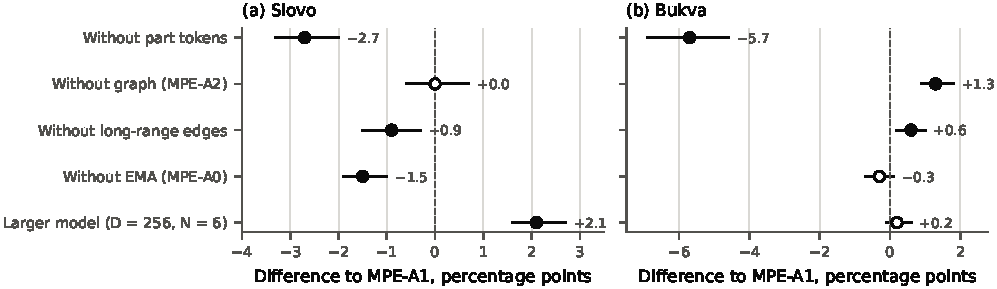
\includegraphics[width=\textwidth]{figures/fig6_ablations.pdf}
\caption{Абляции МПК-A1 по SD-5 (три затравки × пять фолдов): парные разности с МПК-A1 и 95 \% ДИ по тестовым исполнителям. Закрашенные маркеры — интервал не содержит нуля.}\label{fig:fig6_ablations}
\end{figure*}

Токены частей --- не универсальный выигрыш. Когда наше представление из 27 точек с двумя системами координат и маской (шесть каналов) заменяет три исходных канала на входе оригинальных ST-GCN и SL-GCN (общий рецепт, одна затравка), точность на Slovo падает на 1,3 {[}−2,7; −0,0{]} и 3,0 пункта {[}−4,1; −1,8{]} (99 \%-е ДИ) и не меняется на Bukva (+0,8 {[}−0,6; +2,2{]} и +0,6 {[}−0,5; +1,9{]}), так что представление не переносится в графовые сети как «лучший вход». И наоборот, гибрид, сохраняющий блоки SL-GCN и их исходный вход и добавляющий сверху токены частей и Conformer (16,9 млн параметров, одна затравка), на Bukva на 1,7 пункта {[}+0,5; +2,8{]} выше оригинального SL-GCN с тем же входом и рецептом, но не на Slovo (−1,3 {[}−2,6; +0,0{]}), и остаётся на 1,7 пункта {[}−2,8; −0,5{]} ниже оригинального SL-GCN с рецептом авторов на Bukva. На наборе американского жестового языка (ASL) соревнования Google Isolated Sign Language Recognition \citep{2023_kaggle_gislr} (94 477 записей, 250 классов, 21 исполнитель) при пятикратной перекрёстной проверке с непересекающимися исполнителями и тремя затравками МПК-A1 достигает 63,9 \% top-1 в среднем по исполнителям, а удаление токенов частей меняет её на −0,1 {[}−0,6; +0,3{]} (99 \%-й ДИ по исполнителям). Таким образом, токены помогают на двух наборах РЖЯ, где главный признак --- кисти, и нейтральны на большом наборе ASL с сильной моделью, обученной с нуля.

\hypertarget{ux43eux444ux438ux446ux438ux430ux43bux44cux43dux43eux435-ux440ux430ux437ux431ux438ux435ux43dux438ux435-slovo}{%
\subsection{Официальное разбиение Slovo}\label{ux43eux444ux438ux446ux438ux430ux43bux44cux43dux43eux435-ux440ux430ux437ux431ux438ux435ux43dux438ux435-slovo}}

Таблица 4 приводит результаты на официальном разбиении, в котором 3 448 из 5 100 тестовых видео (67,6 \%) принадлежат 92 исполнителям, присутствующим и в обучении. МПК-A1 достигает 64,1 \% {[}61,3; 66,8{]}, что совпадает с 64,09 \%, опубликованными для видеомодели MViTv2-S \citep{2023_kapitanov_slovo}. Запущенная с опубликованным кодом вывода, который зацикливает короткие видео для заполнения входного окна, MViTv2-S достигает лишь 51,4 \% {[}48,3; 54,4{]}; дополнение коротких видео последним кадром воспроизводит опубликованное значение (64,3 \% {[}61,6; 67,1{]}). Мы выбрали эту настройку на 966 тестовых видео; на остальных 4 134 она даёт 64,15 \%, так что воспроизведение --- не артефакт этого выбора. Относительно более сильной настройки парная разность с МПК-A1 составляет −0,2 пункта {[}−2,2; +2,0{]}, то есть различие по точности top-1 не установлено, тогда как у MViTv2-S выше точность top-5 (90,5 \% против 86,6 \%). Опубликованная MViTv2-S имеет 35,0 млн параметров (140,8 МБ в ONNX) и обрабатывает RGB-видео; МПК-A1 --- 3,38 млн (13,5 МБ) и работает по ключевым точкам. Увеличенный МПК достигает 67,0 \%.

\begin{table*}[t]
\caption{Официальное разбиение Slovo (5 100 тестовых видео, 174 исполнителя, 92 из них есть в обучении). Три затравки для моделей по точкам; MViTv2-S — единственная опубликованная модель. P0 — код вывода авторов; R1 — дополнение коротких видео последним кадром.}\label{tab:official}
\footnotesize
\centering
\begin{tabular}{lllrl}
\toprule
\textbf{Модель} & \textbf{Вход} & \textbf{Top-1 [95 \% ДИ]} & \textbf{Top-5} & \textbf{$\Delta$ с МПК-A1} \\
\midrule
МПК-A1 & точки & 64,1 [61,3; 66,8] & 86,6 & --- \\
МПК-A0 & точки & 63,2 [60,1; 65,9] & 85,3 & −1,0 [−1,5; −0,5] \\
МПК-A2 (без графа) & точки & 63,5 [60,6; 66,4] & 87,3 & −0,6 [−1,5; +0,3] \\
МПК, D = 256, N = 6 & точки & 67,0 [64,3; 69,5] & 89,4 & +2,9 [+2,2; +3,6] \\
Трансформер по точкам & точки & 62,2 [59,8; 64,9] & 84,8 & −1,9 [−3,6; −0,3] \\
MViTv2-S, по данным авторов Slovo & RGB-видео & 64,09 & --- & --- \\
MViTv2-S, код авторов (P0) & RGB-видео & 51,4 [48,3; 54,4] & 78,9 & −12,8 [−15,5; −10,3] \\
MViTv2-S, дополнение последним кадром (R1) & RGB-видео & 64,3 [61,6; 67,1] & 90,5 & +0,2 [−2,0; +2,2] \\
MViTv2-S 48/2 (R1) & RGB-видео & 61,9 [59,1; 64,6] & 89,0 & −2,3 [−4,3; −0,2] \\
ResNet-i3d (R1) & RGB-видео & 19,0 [16,2; 22,4] & 37,1 & −45,1 [−48,2; −41,6] \\
\bottomrule
\end{tabular}
\end{table*}

\hypertarget{ux43aux43eux440ux43fux443ux441-ux443ux437ux431ux435ux43aux441ux43aux43eux433ux43e-ux436ux435ux441ux442ux43eux432ux43eux433ux43e-ux44fux437ux44bux43aux430-ux43dux43eux432ux44bux435-ux438ux441ux43fux43eux43bux43dux438ux442ux435ux43bux438}{%
\subsection{Корпус узбекского жестового языка: новые исполнители}\label{ux43aux43eux440ux43fux443ux441-ux443ux437ux431ux435ux43aux441ux43aux43eux433ux43e-ux436ux435ux441ux442ux43eux432ux43eux433ux43e-ux44fux437ux44bux43aux430-ux43dux43eux432ux44bux435-ux438ux441ux43fux43eux43bux43dux438ux442ux435ux43bux438}}

Таблица 5 даёт результаты LOSO, рис. 6 --- точность на каждом отложенном исполнителе. Предобученный на Slovo и Bukva и дообученный на наборе оценки из 682 классов, МПК-A1 достигает на новом исполнителе 32,0 \% {[}25,0; 39,2{]} top-1 и 52,0 \% {[}44,4; 60,0{]} top-5 (микросредние 25,2 \% и 44,3 \%; макро-\(F_1\) 20,5 \%). Обученный с нуля на тех же данных с семикратно большим бюджетом, он достигает 17,3 \% {[}12,3; 23,5{]}: предобучение добавляет 14,7 пункта {[}+11,2; +18,6{]} (99 \%-й ДИ {[}+10,4; +20,0{]}) и помогает каждому из десяти исполнителей. Когда для обучения используются все 5 993 записи и голова из 2 381 класса, выигрыш предобучения составляет 12,2 пункта {[}+7,2; +17,3{]} (девять из десяти исполнителей), но точность на классах оценки падает с 32,0 \% до 26,2 \% (−5,8 {[}−8,0; −3,9{]}, десять из десяти исполнителей): дополнительные классы с одной записью добавляют в голову около 1 700 отвлекающих вариантов, среди них синонимы и альтернативные написания (\emph{shapka} → \emph{telpak}, \emph{sosiska} → \emph{sasiska}, латинские буквы, предсказываемые как их кириллические аналоги), и в разведочной, не предзарегистрированной проверке ограничение ответа классами оценки возвращает всё, кроме 1,1 пункта. Предобучение помогает словам больше, чем дактилю: +15,0 пункта {[}+10,8; +19,7{]} для восьми исполнителей со словами (улучшаются все восемь) и +11,7 пункта {[}+8,3; +16,7{]} для трёх исполнителей с не менее чем десятью дактильными записями.

\begin{table*}[t]
\caption{Корпус УзЖЯ, «исключение одного исполнителя» по десяти исполнителям (три затравки). Top-1 и top-5 — среднее по исполнителям [95 \% ДИ, бутстреп по исполнителям]; top-1 (зап.) — среднее по записям; точность (precision), полнота и $F_1$ — macro по классам; слова / дактиль — top-1, среднее по исполнителям с ≥ 10 записями группы. Голова — число классов обучения.}\label{tab:loso}
\scriptsize\setlength{\tabcolsep}{3pt}
\centering
\begin{tabular}{lllcrrrrrrr}
\toprule
\textbf{Модель} & \textbf{Предобучение} & \textbf{Голова} & \textbf{Top-1 [95 \% ДИ]} & \textbf{Top-1 (зап.)} & \textbf{Top-5} & \textbf{Точность} & \textbf{Полнота} & \textbf{$F_1$} & \textbf{Слова} & \textbf{Дактиль} \\
\midrule
МПК-A1 & Slovo + Bukva & 682 & 32,0 [25,0; 39,2] & 25,2 & 52,0 & 20,9 & 22,7 & 20,5 & 28,0 & 35,0 \\
МПК-A1 & нет & 682 & 17,3 [12,3; 23,5] & 13,0 & 32,2 & 9,9 & 10,9 & 9,4 & 13,0 & 23,3 \\
МПК-A1 & Slovo + Bukva & 2 033–2 378 & 26,2 [20,1; 32,7] & 20,4 & 45,1 & 21,6 & 18,1 & 18,5 & 23,2 & 27,4 \\
МПК-A1 & нет & 2 033–2 378 & 14,0 [8,2; 21,4] & 9,7 & 24,6 & 10,4 & 7,8 & 8,1 & 8,9 & 23,0 \\
SL-GCN (оригинал) & Slovo + Bukva & 682 & 34,9 [26,9; 43,2] & 27,4 & 55,4 & 22,3 & 24,0 & 22,0 & 30,4 & 36,8 \\
МПК-A1 & Slovo + Bukva + ASL & 682 & 30,3 [25,7; 35,0] & 25,5 & 53,0 & 21,3 & 23,0 & 20,9 & 28,9 & 24,9 \\
\bottomrule
\end{tabular}
\end{table*}

\begin{figure*}[t]
\centering
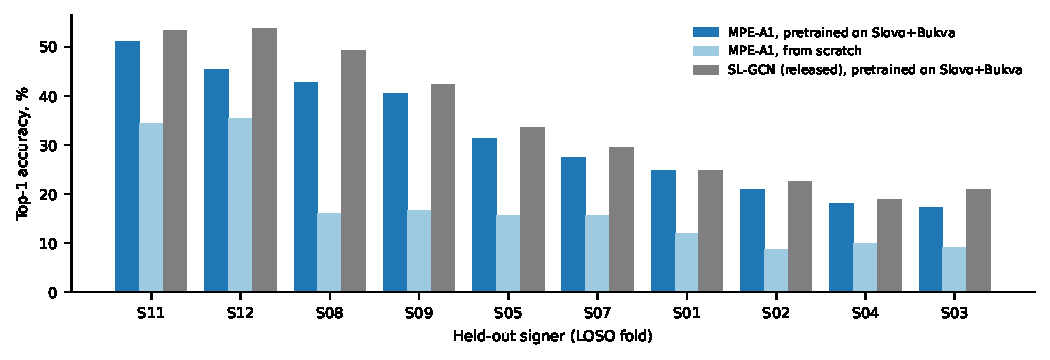
\includegraphics[width=\textwidth]{figures/fig_loso_signers.pdf}
\caption{Корпус УзЖЯ: точность top-1 на каждом отложенном исполнителе (LOSO, среднее трёх затравок) для МПК-A1 с предобучением на Slovo + Bukva, МПК-A1 с нуля и оригинального SL-GCN с предобучением на Slovo + Bukva (набор оценки, 682 класса).}\label{fig:fig_loso_signers}
\end{figure*}

Оригинальный SL-GCN, предобученный и дообученный по точно такому же протоколу, достигает 34,9 \% {[}26,9; 43,2{]}: на 2,9 пункта {[}+1,5; +4,5{]} выше МПК-A1 (99 \%-й ДИ {[}+1,3; +5,1{]}), выше у девяти из десяти исполнителей, что повторяет порядок, наблюдавшийся на Slovo (SL-GCN не обучался на корпусе с нуля; на пилоте с нуля он намного слабее МПК-A1, раздел 6.6). Точность у обеих моделей сильно различается между исполнителями --- от 17 \% до 51 \% для МПК-A1; два участника пилота, чьи записи --- чистый дактиль, самые лёгкие, а среди ведущих уроков точность меняется от 17 \% (S03) до 43 \% (S08) и не объясняется одним лишь размером словаря. Самые частые путаницы после предобучения --- между буквами и словами со сходной формой кисти (\emph{Gʻ} → \emph{G}, \emph{E} → \emph{may}, \emph{U} → \emph{qayerga}) и между близкими синонимами (\emph{blinchik} → \emph{quymoq}, \emph{likopcha} → \emph{tarelka}, \emph{ona} → \emph{ayol}); полный список приведён в дополнительных материалах.

\hypertarget{ux432ux43dux435ux448ux43dux438ux435-ux438ux441ux442ux43eux447ux43dux438ux43aux438-1}{%
\subsection{Внешние источники}\label{ux432ux43dux435ux448ux43dux438ux435-ux438ux441ux442ux43eux447ux43dux438ux43aux438-1}}

Таблица 6 приводит результаты итоговых моделей, обученных один раз с затравкой 0 на всём корпусе, на двух внешних источниках без какой-либо подстройки. На 93 видео N01, чей жест входит в 682 класса оценки, предобученная модель достигает 33,3 \% {[}23,7; 43,0{]} top-1 и 53,8 \% top-5 (интервалы по записям, поскольку у источника один ведущий); на 199 видео словаря, метка которых точно совпадает с одним из 181 класса оценки, --- 33,7 \% {[}26,9; 40,5{]} и 60,2 \% (точность усреднена по словам; интервалы по словам). Оценка LOSO в 32,0 \% таким образом воспроизводится на двух независимых источниках с новыми людьми, новыми камерами и метками, которые делали не мы. Выигрыш предобучения тоже воспроизводится: с головой из 2 381 класса предобучение поднимает точность top-1 с 9,3 \% до 24,0 \% на N01 (+14,7 {[}+6,7; +22,7{]} по 150 видео) и с 6,7 \% до 15,9 \% на словаре (+9,2 {[}+5,4; +12,9{]} по 356 словам). Добавление набора ASL к источникам предобучения даёт 38,7 \% на словаре, +5,0 пункта {[}−1,5; +11,5{]} относительно одних Slovo и Bukva, и никаких изменений на N01 (+0,0 {[}−10,8; +10,8{]}), так что польза третьего языка-источника не установлена.

\begin{table*}[t]
\caption{Внешние источники, итоговые модели на всём корпусе (одна затравка), без подстройки. Оцениваются только видео, чей знак входит в голову модели; для словаря — только видео, метка которых точно совпадает с классом корпуса, точность усреднена по словам. Интервалы — бутстреп по записям (N01, один ведущий) или по словам (словарь).}\label{tab:external}
\footnotesize
\centering
\begin{tabular}{llrrrlr}
\toprule
\textbf{Источник} & \textbf{Модель} & \textbf{Голова} & \textbf{Видео} & \textbf{Слов} & \textbf{Top-1 [95 \% ДИ]} & \textbf{Top-5} \\
\midrule
N01 & предобучение (Slovo + Bukva) & 682 & 93 & 93 & 33,3 [23,7; 43,0] & 53,8 \\
N01 & предобучение (Slovo + Bukva + ASL) & 682 & 93 & 93 & 33,3 [23,7; 43,0] & 68,8 \\
N01 & предобучение, все записи & 2 381 & 150 & 150 & 24,0 [17,3; 30,7] & 40,7 \\
N01 & с нуля, все записи & 2 381 & 150 & 150 & 9,3 [4,7; 14,0] & 18,0 \\
imo-ishora.uz & предобучение (Slovo + Bukva) & 682 & 199 & 181 & 33,7 [26,9; 40,5] & 60,2 \\
imo-ishora.uz & предобучение (Slovo + Bukva + ASL) & 682 & 199 & 181 & 38,7 [31,7; 45,9] & 64,6 \\
imo-ishora.uz & предобучение, все записи & 2 381 & 397 & 356 & 15,9 [12,3; 19,8] & 36,4 \\
imo-ishora.uz & с нуля, все записи & 2 381 & 397 & 356 & 6,7 [4,4; 9,4] & 16,0 \\
\bottomrule
\end{tabular}
\end{table*}

\hypertarget{ux43fux438ux43bux43eux442ux43dux44bux435-ux437ux430ux43fux438ux441ux438-ux431ux44eux434ux436ux435ux442ux44b-ux437ux430ux434ux430ux43dux43dux44bux435-ux437ux430ux440ux430ux43dux435ux435-ux438-ux43eux43fux442ux438ux43cux438ux437ux43c-ux432ux43dux443ux442ux440ux438-ux438ux441ux43fux43eux43bux43dux438ux442ux435ux43bux44f}{%
\subsection{Пилотные записи: бюджеты, заданные заранее, и оптимизм внутри исполнителя}\label{ux43fux438ux43bux43eux442ux43dux44bux435-ux437ux430ux43fux438ux441ux438-ux431ux44eux434ux436ux435ux442ux44b-ux437ux430ux434ux430ux43dux43dux44bux435-ux437ux430ux440ux430ux43dux435ux435-ux438-ux43eux43fux442ux438ux43cux438ux437ux43c-ux432ux43dux443ux442ux440ux438-ux438ux441ux43fux43eux43bux43dux438ux442ux435ux43bux44f}}

Пилотный набор повторяет эксперимент по переносу в контролируемом масштабе --- с двумя тестовыми участниками и бюджетами обучения, зафиксированными до первого запуска (таблица 7, рис. 7б). Обученный с нуля, МПК-A1 достигает 9,5 \%, 11,7 \% и 24,7 \% при одном примере на класс, двух примерах на класс и всех записях (объединённо по двум тестовым участникам). Каждое условие с предобучением лучше обучения с нуля на той же ступени во всех шести парах «затравка--фолд», 18 из 18 сравнений; лучшие объединённые точности, со Slovo и Bukva вместе и полным дообучением, --- 40,3 \%, 41,2 \% и 47,5 \%. Поскольку часть тестовых классов отсутствует в обучающих данных фолда, эти точности ограничены сверху 82,5 \% для участника 002 и 67,0 \% для участника 003. Линейный зонд близок к полному дообучению (45,4 \% против 47,5 \%), лучший источник у участников различается, а МПК-A2 без графа переносится не хуже МПК-A1 (47,9 \% с зондом; знак его разности непостоянен). Оригинальный SL-GCN, перенесённый по тому же протоколу, чуть менее точен, чем МПК-A1, после полного дообучения (45,9 \%, ниже во всех шести парах) и точнее как замороженный кодировщик (49,8 \% против 45,4 \%, выше в пяти парах при одной ничьей, то есть по правилу не установлено). Матрица ошибок букв пилота (рис. 9б) показывает, что ошибки сосредоточены на буквах, визуально близких в дактиле УзЖЯ (\emph{Gʻ} → \emph{G}, \emph{CH} → \emph{A}/\emph{J}, \emph{E} → \emph{X}/\emph{Y}), и на числительных, которые встречаются в записях только одного участника.

\begin{table*}[t]
\caption{Пилот УзЖЯ с бюджетами, заданными заранее (МПК-A1, если не указано; три затравки × два фолда): top-1 по записям обоих тестовых участников, в скобках — участники 002 / 003. Каждое условие с предобучением лучше обучения с нуля на той же ступени во всех шести парах.}\label{tab:pilot}
\footnotesize
\centering
\begin{tabular}{lllll}
\toprule
\textbf{Предобучение} & \textbf{Схема} & \textbf{Один пример на класс} & \textbf{Два примера на класс} & \textbf{Все записи} \\
\midrule
Нет & с нуля & 9,5 (12,8 / 6,8) & 11,7 (9,8 / 13,3) & 24,7 (21,0 / 27,6) \\
Slovo & линейный зонд & 31,0 (38,7 / 24,8) & 37,7 (42,7 / 33,7) & 41,2 (43,1 / 39,6) \\
Slovo & дообучение & 31,7 (35,2 / 28,8) & 33,9 (38,7 / 29,9) & 39,4 (42,0 / 37,3) \\
Bukva & линейный зонд & 27,5 (33,6 / 22,5) & 39,2 (45,0 / 34,5) & 46,1 (49,6 / 43,2) \\
Bukva & дообучение & 35,6 (40,6 / 31,6) & 38,5 (41,5 / 36,0) & 46,3 (50,4 / 43,0) \\
Slovo + Bukva & линейный зонд & 37,2 (46,4 / 29,7) & 39,4 (47,1 / 33,1) & 45,4 (49,9 / 41,7) \\
Slovo + Bukva & дообучение & 40,3 (48,5 / 33,7) & 41,2 (46,9 / 36,5) & 47,5 (49,9 / 45,6) \\
Slovo + Bukva, МПК-A2 & линейный зонд & 38,0 (44,8 / 32,6) & 40,3 (45,9 / 35,8) & 47,9 (52,7 / 43,9) \\
Slovo + Bukva, МПК-A2 & дообучение & 35,4 (36,1 / 34,9) & 40,5 (42,9 / 38,6) & 45,8 (47,1 / 44,7) \\
Slovo + Bukva, SL-GCN (оригинал) & линейный зонд & 41,3 (49,9 / 34,3) & 47,2 (54,1 / 41,7) & 49,8 (56,2 / 44,7) \\
Slovo + Bukva, SL-GCN (оригинал) & дообучение & 34,2 (34,5 / 33,9) & 39,5 (36,8 / 41,7) & 45,9 (47,1 / 44,9) \\
Нет, SL-GCN (оригинал) & с нуля & 5,5 (7,5 / 4,0) & 5,3 (3,0 / 7,2) & 15,2 (8,6 / 20,4) \\
\bottomrule
\end{tabular}
\end{table*}

\begin{figure*}[t]
\centering
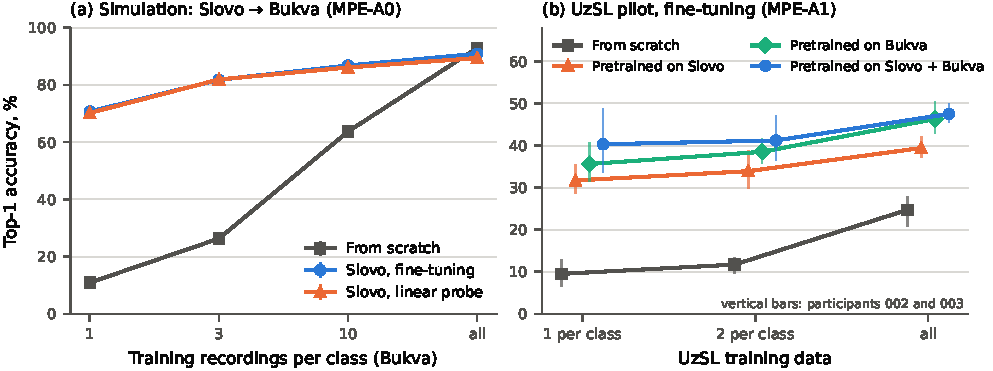
\includegraphics[width=\textwidth]{figures/fig7_transfer.pdf}
\caption{Перенос с РЖЯ. (а) Моделирование на Bukva по SD-5 (МПК-A0): точность top-1 при 1, 3 и 10 обучающих записях на класс и при всех записях, с нуля и после предобучения на Slovo; отрезки — 95 \% ДИ по исполнителям. (б) Пилот УзЖЯ (МПК-A1, полное дообучение): top-1 по записям обоих тестовых участников при одном и двух примерах на класс и при всех записях; вертикальные отрезки охватывают двух участников.}\label{fig:fig7_transfer}
\end{figure*}

Моделирование на Bukva по SD-5 показывает тот же эффект при многих тестовых исполнителях (рис. 7а): предобучение на Slovo поднимает точность с 10,9 \% до 70,7 \% при одной обучающей записи на класс (+59,7 {[}+57,8; +61,5{]}), с 26,3 \% до 81,8 \% при трёх и с 63,7 \% до 86,8 \% при десяти, тогда как при всех обучающих данных Bukva оно слегка вредит (90,9 \% против 92,9 \%, −2,0 {[}−2,8; −1,2{]}); польза предобучения уменьшается и может смениться на обратную, когда целевых данных достаточно.

\textbf{Валидация на обучающих участниках завышает точность.} До того как бюджеты были зафиксированы, наши первые опыты на пилоте выбирали контрольные точки по отложенным записям обучающих участников. Рис. 8 сравнивает для 23 условий этих опытов валидационную точность в выбранной контрольной точке с точностью на новом участнике: валидационная точность лежала от 54 \% до 100 \%, тестовая --- от 7 \% до 51 \%, а разрыв имел медиану 45,2 пункта (размах 35,0--75,1), наибольший при обучении с нуля. Модель, видевшая участника, почти безошибочна на его новых записях и теряет половину точности или больше на новом участнике. Поэтому все результаты на пилоте и корпусе используют заданные заранее бюджеты и последнюю контрольную точку, и поэтому точности, полученные при пересечении исполнителей, включая опубликованные до сих пор для УзЖЯ, следует читать как верхние границы.

\begin{figure*}[t]
\centering
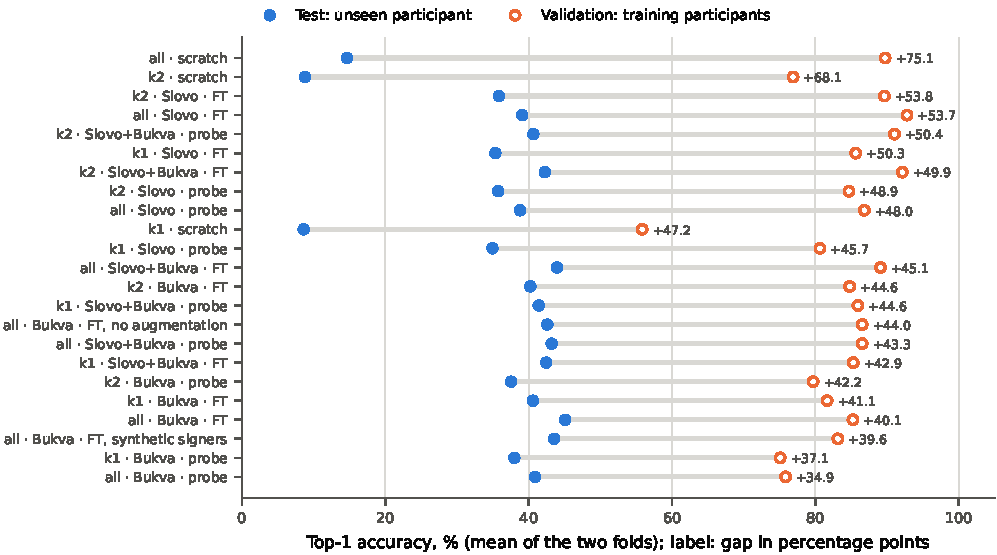
\includegraphics[width=\textwidth]{figures/fig8_valtest.pdf}
\caption{Валидационная точность на отложенных записях участников обучения (в выбранной контрольной точке) и тестовая точность на новом участнике для 23 условий первых опытов на пилоте (МПК-A0), среднее по двум фолдам, по убыванию разрыва. k1, k2 — один и два примера на класс; all — все записи; FT — полное дообучение; probe — линейный зонд.}\label{fig:fig8_valtest}
\end{figure*}

\hypertarget{ux443ux441ux442ux43eux439ux447ux438ux432ux43eux441ux442ux44c-ux438-ux432ux43dux435ux434ux440ux435ux43dux438ux435}{%
\subsection{Устойчивость и внедрение}\label{ux443ux441ux442ux43eux439ux447ux438ux432ux43eux441ux442ux44c-ux438-ux432ux43dux435ux434ux440ux435ux43dux438ux435}}

Таблица 8 приводит точность, когда ведущая кисть удалена из доли \(p\) кадров и когда к ключевым точкам добавлен гауссов шум со стандартным отклонением \(\sigma\) (в долях ширины кадра), для контрольных точек SD-5 без переобучения. Удаление ведущей кисти из четверти кадров не меняет МПК-A1 (при обучении кисть выбрасывается в 20--25 \% кадров); удаление из половины кадров стоит 1,5 пункта на Slovo и 1,0 на Bukva. Шум --- более сильный фактор: \(\sigma\) = 0,02 стоит 6,4 пункта на Slovo и 4,2 на Bukva. МПК-A2 устойчивее к шуму на обоих наборах (+2,4 и +3,4 пункта при \(\sigma\) = 0,02) и чуть чувствительнее к отсутствию кистей на Slovo.

\begin{table*}[t]
\caption{Точность top-1 МПК-A1 и МПК-A2 при искажении точек (SD-5, три затравки × пять фолдов). $p$ — доля кадров без ведущей кисти; $\sigma$ — гауссов шум в долях ширины кадра; $\Delta$ — парная разность A2 − A1 [95 \% ДИ].}\label{tab:robustness}
\small
\centering
\begin{tabular}{lrrlrrl}
\toprule
\textbf{Искажение} & \textbf{Slovo A1} & \textbf{Slovo A2} & \textbf{$\Delta$ Slovo} & \textbf{Bukva A1} & \textbf{Bukva A2} & \textbf{$\Delta$ Bukva} \\
\midrule
Нет & 70,8 & 70,8 & +0,0 [−0,7; +0,7] & 93,2 & 94,5 & +1,3 [+0,9; +1,8] \\
$p = 0,25$ & 70,7 & 70,2 & −0,5 [−1,2; +0,2] & 93,3 & 94,0 & +0,7 [+0,3; +1,2] \\
$p = 0,5$ & 69,3 & 68,0 & −1,3 [−2,1; −0,5] & 92,2 & 93,0 & +0,8 [+0,3; +1,4] \\
$\sigma = 0,01$ & 70,0 & 69,8 & −0,2 [−1,0; +0,5] & 92,4 & 93,9 & +1,6 [+1,0; +2,1] \\
$\sigma = 0,02$ & 64,4 & 66,7 & +2,4 [+1,2; +3,6] & 89,0 & 92,4 & +3,4 [+2,7; +4,1] \\
$p = 0,5$, $\sigma = 0,02$ & 59,4 & 60,9 & +1,5 [−0,1; +3,0] & 87,6 & 90,5 & +2,9 [+2,1; +3,6] \\
\bottomrule
\end{tabular}
\end{table*}

Экспортированный в TensorFlow Lite (float32), МПК-A1 занимает 12,5 МиБ и выполняется за 24,4 мс на окно из 32 кадров на настольном ЦП при числе потоков по умолчанию (29,1 мс в один поток) с тем же argmax, что и модель PyTorch, на всех 1 051 проверенной записи; МПК-A2 без графа занимает 11,6 МиБ и выполняется за 6,6 мс. Экспорт МПК-A1 в ONNX с тремя головами --- 13,5 МБ; задержки в ONNX Runtime приведены в разделе 6.1. Задержка на телефоне не измерялась.

\begin{figure*}[t]
\centering
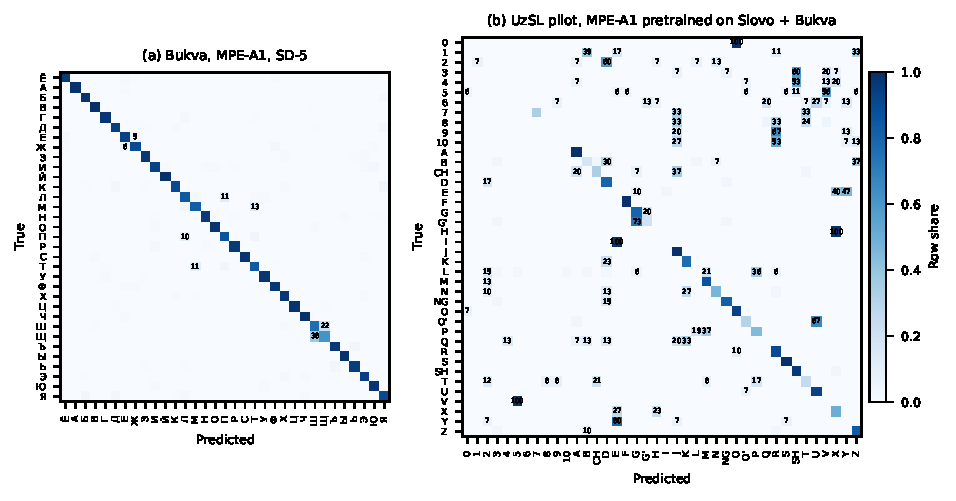
\includegraphics[width=\textwidth]{figures/fig_confusions.pdf}
\caption{Матрицы ошибок (строки нормированы; подписаны внедиагональные ячейки ≥ 5 \%). (а) Bukva, МПК-A1 по SD-5, 33 буквы дактильной азбуки РЖЯ. (б) Пилот УзЖЯ, МПК-A1 с предобучением на Slovo + Bukva и дообучением на всех записях, 29 букв и 11 цифр; цифры и буквы H, I, Q, V, Y есть только у одного участника и потому отсутствуют в обучении своего тестового фолда.}\label{fig:fig_confusions}
\end{figure*}

\hypertarget{ux43eux431ux441ux443ux436ux434ux435ux43dux438ux435}{%
\section{Обсуждение}\label{ux43eux431ux441ux443ux436ux434ux435ux43dux438ux435}}

\textbf{Что означают первые независимые от исполнителя числа для УзЖЯ.} Изолированный жест нового исполнителя распознаётся верно примерно в трети случаев и попадает в пять кандидатов примерно в половине --- на словаре из 682 классов, выученных по медиане из четырёх записей на класс. Эти числа нельзя сравнивать с 87--99 \%, сообщавшимися для УзЖЯ до сих пор: те измерены на исполнителях, присутствовавших в обучении, на закрытых наборах из 50 или менее классов либо неизвестного состава, а пилотный эксперимент раздела 6.6 показывает, чего стоит такое измерение (медиана оптимизма --- 45 пунктов). Оценка LOSO подтверждена двумя внешними источниками, поэтому она честно описывает текущее состояние и задаёт задачу следующему поколению распознавателей УзЖЯ: не выше точность на виденных исполнителях, а выше точность на новых.

\textbf{Предобучение на родственном жестовом языке --- главный рычаг.} На корпусе (+14,7 пункта, у каждого исполнителя), на двух внешних источниках (+9,2 и +14,7 пункта), на пилоте (18 из 18 сравнений) и в моделировании на Bukva (+59,7 пункта при одной записи на класс) предобучение на РЖЯ --- единственное вмешательство, которое помогает всегда, и помогает больше всего там, где целевых данных меньше всего. Словам оно помогает больше, чем дактилю, что согласуется с тем, что дактильные азбуки двух языков различаются формой нескольких букв, тогда как лексиконы пересекаются. Эти результаты поддерживают гипотезу о переносе представлений РЖЯ на УзЖЯ; они не устанавливают лингвистического родства языков, а третий, неродственный источник (ASL) не добавляет ничего, что могли бы установить данные.

\textbf{Архитектура значит меньше, чем подсказывают оригинальные базовые модели.} На Slovo, на корпусе и на пилоте в качестве замороженного кодировщика оригинальный SL-GCN на 2--4 пункта точнее нашего кодировщика; МПК --- более дешёвая модель, а не более точная, и его ценность --- в точности, достигаемой при 0,76 GFLOPs (0,196 GFLOPs без графа), в анализе того, какие компоненты важны, и в переносе, где после полного дообучения он не уступает. Абляции указывают на один структурный элемент --- группировку ключевых точек в токены частей тела с собственными системами координат; скелетный граф можно заменить MLP по частям без потерь. Те же токены нейтральны на большом наборе ASL, так что их польза привязана к режиму малого числа записей на класс и жестов, определяемых кистями. Важнее для области разрыв в 4--9 пунктов между нашими реализациями ST-GCN и SL-GCN и их оригинальным кодом: сравнение с переписанными базовыми моделями перевернуло бы вывод этой статьи. Базовые модели следует запускать из оригинального кода везде, где он есть, а переписанные реализации --- помечать как таковые.

\textbf{Практика оценки.} Два измерения показывают, как сильно пересечение исполнителей влияет на сообщаемую точность: медианный разрыв в 45 пунктов между валидацией на обучающих участниках и тестом на новом и две трети официального тестового набора Slovo, принадлежащие обучающим исполнителям. Задание бюджетов по моделированию со многими исполнителями и оценка последней контрольной точки, как сделано здесь для пилота и корпуса, --- практичная замена валидационного набора, когда у целевого языка лишь несколько исполнителей.

\textbf{Внедрение.} По числу операций МПК в 2,6--2,9 раза дешевле графовых сетей при том же окне и в 12,8 раза дешевле SL-GCN при его собственном тестовом окне, а его экспорт в TensorFlow Lite выполняется за 24 мс (6,6 мс без графа) на настольном ЦП; в ONNX Runtime он быстрее обеих графовых сетей (10,8 против 15,0 и 25,6 мс в один поток), однако в eager-режиме PyTorch он не быстрее ST-GCN, а измерений на телефоне пока нет. Число операций с плавающей точкой --- неполный заменитель задержки, и среда выполнения меняет порядок моделей; итоговую модель нужно измерять на том устройстве и в той среде, где она будет работать.

\textbf{Ограничения.} Корпус построен из уроков: у каждого ведущего одна студия и одна камера, поэтому LOSO измеряет нового человека вместе с новыми условиями съёмки, а три самых больших словаря принадлежат трём ведущим. Автоматические метки проверены по словарю для 113 записей одним проверяющим; точность на словах, отсутствующих в словаре, опирается на суждение проверяющего, а запланированная вторая выборка записей уроков и второй проверяющий ещё впереди. Синонимы и дубликаты в латинице и кириллице --- отдельные классы, что снижает точность при полной голове. Корпус не может быть опубликован, поскольку видеоуроки и извлечённые из них точки идентифицируют ведущих; вместо него публикуются код, списки фолдов и процедура построения. У пилота два основных участника, записанные за один сеанс. Оригинальные ST-GCN и SL-GCN и МПК-A1 с рецептом SL-GCN запускались с одной затравкой на SD-5, а у трансформера по ключевым точкам и простых базовых моделей нет оригинальных аналогов. Абляции, исследование ёмкости и проверки устойчивости выполнены только на данных РЖЯ; проверка устойчивости использует независимый синтетический шум, который лишь приближает коррелированные во времени ошибки реального детектора точек, а смена экстрактора точек не проверялась.

\hypertarget{ux437ux430ux43aux43bux44eux447ux435ux43dux438ux435}{%
\section{Заключение}\label{ux437ux430ux43aux43bux44eux447ux435ux43dux438ux435}}

Это исследование даёт первые результаты распознавания узбекского жестового языка, полученные на исполнителях, отсутствующих в обучении, и показывает, чем они определяются. Многопользовательский корпус, построенный из открытых видеоуроков с метками, проверенными по словарю, делает возможной оценку на новых исполнителях; на нём компактный кодировщик ключевых точек распознаёт жест нового исполнителя с точностью 32,0 \% top-1 и 52,0 \% top-5 на 682 классах --- оценка, воспроизведённая на двух внешних источниках. Предобучение на двух открытых наборах русского жестового языка повышает точность у каждого отложенного исполнителя --- на 14,7 пункта на корпусе и на 23 пункта на пилоте --- и является главным рычагом, доступным жестовому языку с малыми ресурсами. На русских наборах по протоколу с непересекающимися исполнителями и предзарегистрированными правилами решения оригинальные графовые сети на 2--4 пункта точнее кодировщика при в 2,6--2,9 раза большем объёме вычислений, тогда как переписанные реализации тех же сетей занижают их на 4--9 пунктов; точность кодировщика обеспечивают токены частей тела, а не скелетный граф, и граф можно убрать, сократив вычисления в 3,9 раза. Наконец, валидация на записях обучающих участников завышает точность на новом исполнителе в медиане на 45 пунктов. Для жестовых языков с малыми ресурсами то, как оценивается система, на чём она предобучена и запущены ли её базовые модели из оригинального кода, важнее её архитектуры. Следующие шаги --- второй проверяющий и большая эталонная выборка для меток, объединение синонимов, проверенное носителем жестового языка, больше исполнителей по той же процедуре построения, распознавание с возможностью отказа для нового исполнителя и измерение задержки на телефонах.

\hypertarget{ux432ux43aux43bux430ux434-ux430ux432ux442ux43eux440ux43eux432-credit}{%
\section{Вклад авторов (CRediT)}\label{ux432ux43aux43bux430ux434-ux430ux432ux442ux43eux440ux43eux432-credit}}

\textbf{Максаджон К. Онаркулов:} концептуализация, научное руководство, написание --- рецензирование и редактирование, администрирование проекта. \textbf{Мирсаид А. Юсупов:} концептуализация, методология, программное обеспечение, валидация, исследование, курирование данных, написание --- первоначальный вариант, написание --- рецензирование и редактирование, визуализация.

\hypertarget{ux434ux435ux43aux43bux430ux440ux430ux446ux438ux44f-ux43e-ux43aux43eux43dux444ux43bux438ux43aux442ux435-ux438ux43dux442ux435ux440ux435ux441ux43eux432}{%
\section{Декларация о конфликте интересов}\label{ux434ux435ux43aux43bux430ux440ux430ux446ux438ux44f-ux43e-ux43aux43eux43dux444ux43bux438ux43aux442ux435-ux438ux43dux442ux435ux440ux435ux441ux43eux432}}

Авторы заявляют об отсутствии известных им конкурирующих финансовых интересов или личных отношений, которые могли бы повлиять на работу, представленную в этой статье.

\hypertarget{ux444ux438ux43dux430ux43dux441ux438ux440ux43eux432ux430ux43dux438ux435}{%
\section{Финансирование}\label{ux444ux438ux43dux430ux43dux441ux438ux440ux43eux432ux430ux43dux438ux435}}

Исследование не получало специального гранта от финансирующих организаций государственного, коммерческого или некоммерческого секторов.

\hypertarget{ux44dux442ux438ux447ux435ux441ux43aux43eux435-ux437ux430ux44fux432ux43bux435ux43dux438ux435}{%
\section{Этическое заявление}\label{ux44dux442ux438ux447ux435ux441ux43aux43eux435-ux437ux430ux44fux432ux43bux435ux43dux438ux435}}

В исследовании участвовали люди. ⟦Одобрение протокола исследования и использования пилотных записей выдано ⟦этическим комитетом / учёным советом Ферганского государственного университета⟧, решение № ⟦\ldots⟧ от ⟦\ldots⟧.⟧ Все участники пилота дали письменное информированное согласие на запись, на использование их данных в исследованиях и на публикацию изображений в научных статьях. Видео уроков и словаря опубликованы открыто; они использованы только для извлечения признаков и оценки, не распространяются, а ведущие обозначены кодами.

\hypertarget{ux434ux43eux441ux442ux443ux43fux43dux43eux441ux442ux44c-ux434ux430ux43dux43dux44bux445}{%
\section{Доступность данных}\label{ux434ux43eux441ux442ux443ux43fux43dux43eux441ux442ux44c-ux434ux430ux43dux43dux44bux445}}

Наборы Slovo и Bukva доступны у их авторов. Пилотные записи УзЖЯ и корпус уроков содержат персональные данные и не передаются; списки фолдов, процедура построения, конфигурации всех экспериментов и код кодировщика, базовых моделей и анализа доступны по адресу https://github.com/M1rsaiD/mpe-slovo-bukva.

\hypertarget{ux434ux435ux43aux43bux430ux440ux430ux446ux438ux44f-ux43eux431-ux438ux441ux43fux43eux43bux44cux437ux43eux432ux430ux43dux438ux438-ux433ux435ux43dux435ux440ux430ux442ux438ux432ux43dux43eux433ux43e-ux438ux438-ux438-ux442ux435ux445ux43dux43eux43bux43eux433ux438ux439-ux441-ux43fux43eux434ux434ux435ux440ux436ux43aux43eux439-ux438ux438-ux432-ux43fux440ux43eux446ux435ux441ux441ux435-ux43dux430ux43fux438ux441ux430ux43dux438ux44f}{%
\section{Декларация об использовании генеративного ИИ и технологий с поддержкой ИИ в процессе написания}\label{ux434ux435ux43aux43bux430ux440ux430ux446ux438ux44f-ux43eux431-ux438ux441ux43fux43eux43bux44cux437ux43eux432ux430ux43dux438ux438-ux433ux435ux43dux435ux440ux430ux442ux438ux432ux43dux43eux433ux43e-ux438ux438-ux438-ux442ux435ux445ux43dux43eux43bux43eux433ux438ux439-ux441-ux43fux43eux434ux434ux435ux440ux436ux43aux43eux439-ux438ux438-ux432-ux43fux440ux43eux446ux435ux441ux441ux435-ux43dux430ux43fux438ux441ux430ux43dux438ux44f}}

При подготовке этой работы авторы использовали Claude (Anthropic) \citep{2026_anthropic_claude} для составления и редактирования текста всех разделов на основе плана исследования, решений и экспериментальных результатов авторов, для написания и отладки кода экспериментов и анализа, для построения рисунков кодом и для проверки библиографических данных; мультимодальная модель той же системы проверяла автоматически сегментированные записи уроков, как описано в разделе 3.3. После использования этого инструмента авторы просмотрели и отредактировали содержание по мере необходимости и несут полную ответственность за содержание публикации. Фотографии на рис. 1 и 3 --- неизменённые кадры видео.

\hypertarget{ux431ux43bux430ux433ux43eux434ux430ux440ux43dux43eux441ux442ux438}{%
\section{Благодарности}\label{ux431ux43bux430ux433ux43eux434ux430ux440ux43dux43eux441ux442ux438}}

Авторы благодарят участников пилотных записей UZSign.AI, а также авторов открытых уроков УзЖЯ и словаря imo-ishora.uz.
